\section*{Learning Objectives}
\begin{itemize}
\item Instead of working with individual vectors, we will work with a collection of vectors. 
\item Our first encounter with some of the essential concepts in Linear Algebra that go beyond systems of equations.
\end{itemize}

\section*{Outcomes}
\begin{itemize}
\item Vectors as $n$-tuples of real numbers
\item $\real^n$ as the collection of all $n$-tuples of real numbers
\item Linear combinations of vectors
\item Linear independence of vectors
\item Relation of these concepts to the existence and uniqueness of solutions to $Ax=b$.
\item How the LU Factorization makes it very straightforward to check the linear independence of a set of vectors, and how a small modification to the LU factorization makes it equally straightforward to check if one vector is a linear combination of a set of vectors. 
\end{itemize}

\vspace*{1cm}

\begin{tcolorbox}[sharp corners, colback=yellow!30, colframe=yellow!80!red, title=\textcolor{red}{\Large \bf Warning! Theory Ahead!! Additional Study Time May Be Required}] 
\bf For many students, the concepts in Chapters \ref{chap:Chap07VectorSpaceRnPart1}, \ref{chap:Rnpart2} and \ref{chap:matrixFacts} are significantly more challenging than the material in any of the other chapters of the book. Why? Well, the reasons vary from person to person, but the biggest reason seems to be the level of abstraction. All of our previous work has pretty much dealt with solving equations and that is something most students of ROB 101 can wrap their heads around. \\

To be considered knowledgeable in Linear Algebra, you need to understand
\begin{itemize}
    \item Linear Combinations and Linear Independence of Vectors
    \item Subspaces
     \item Span of a set of vectors
    \item Basis vectors and coordinates
    \item Dimension of a subspace
    \item Relations of the above to Matrices
\end{itemize}

\end{tcolorbox}


\newpage

\section{Motivation}

At this point, if we have a matrix equation, $Ax=b$, we understand that $\bar{x}$ is a solution to the equation if, and only if, $A\bar{x}-b=0$; in other words, plugging $\bar{x}$ into the equation results in there being ``no error.'' In this chapter, we are setting ourselves up for deeper questions, such as what is the set of all solutions to an equation of the form $Ax=b$? What does it even mean to talk about ``all solutions'' to an equation? \\

To make this last question a bit more concrete, let's suppose that we have found two solutions to the equation $Ax=0_{n \times 1}$ (yes, we took $b=0_{n \times 1}$), and we call them $\bar{x}$ and  $\bar{\bar{x}}$. We now let $\alpha \in \real$ and $\beta \in \real$ be two real numbers and we define a third potential solution by 
\begin{equation}
\label{eq:FirstLinearCombo}
   \check x := \alpha \bar{x} + \beta \bar{\bar{x}}.  
\end{equation}
Is there any chance it is really a solution? In other words, just by doing simple algebraic operations on existing solutions, can we find other solutions? Let's find out by plugging $\check x$ into the equation,
\begin{align*}
    A \check x & = A \left( \alpha \bar{x} + \beta \bar{\bar{x}} \right) \\
    & = A \left(\alpha \bar{x}\right) + A \left(\beta \bar{\bar{x}} \right)\\
    & =  \alpha A \bar{x} + \beta A \bar{\bar{x}} \\
    &= 0 + 0\\
    &=0.
\end{align*}
Bingo, $\check x$ is also a solution. Since there can be more than one solution, we are motivated to define
\begin{equation}
\label{eq:FirstSetAllSolutions}
    S_{\rm all}:=\{ x~|~ A x =0_{n \times 1} \}, 
\end{equation}
the set of all possible solutions. Assuming we could compute such a set, what would we even do with it? Later in the course, we'll define what it means to say that one vector $\bar{x} \in S_{\rm all}$ is ``better than'' another vector $\bar{\bar x} \in S_{\rm all}$, in other words, we'll define what it means for one solution (to an engineering problem) to be better than another solution (to an engineering problem). If you can compare one solution to another, then you can potentially quantify what is a ``best'' solution to a problem! For example, we could potentially pose problems about how to go from point $A$ to point $B$ using the least amount of energy, or how to manufacture something at lowest cost.\\

We're straying a bit from Linear Algebra here, but hopefully, the teaser was kind of fun. We summarize:
\begin{itemize}
    \item It makes sense to perform algebraic operations on solutions of equations, as in \eqref{eq:FirstLinearCombo}.
    \item It is at least plausible that understanding the ``structure'' of abstract sets like \eqref{eq:FirstSetAllSolutions} will make it easier to sort through the set to find a ``best element'' in the set, when later in the course, we are able to define what we mean by ``best''!
\end{itemize}

\begin{tcolorbox}[title=\textcolor{red}{\bf \Large Need Intuition?}]
 The YouTube Channel \textbf{3Blue1Brown} has a video series on the ``essence'' of Linear Algebra. Here is one you may like which talks about vectors, points, and coordinates \url{https://youtu.be/fNk_zzaMoSs}; there are many others. The series has wonderful animations. \textbf{If you find yourself struggling with the abstract concepts we are about to encounter, then this video series may be for you!} Others of you will not need the animations and the fact that the animations have to be done in dimensions two and three may actually inhibit you from mastering the material. We all learn in different ways. 
\end{tcolorbox}



\section{Vectors in $\real^n$ and Some Basic Algebra}

An $n$-tuple is a fancy name for an ordered list of $n$ numbers, $(x_1, x_2, \ldots, x_n)$. If this sounds a lot like a vector, then good, because \textbf{we will systematically identify}
\begin{equation}
\real^n:=\{(x_1, x_2, \ldots, x_n)~|~x_i \in \real, 1\le i \le n \} 
\end{equation}
\textbf{with column vectors}. In other words, for us,
\begin{equation}
\real^n:=\{(x_1, x_2, \ldots, x_n)~|~x_i \in \real, 1\le i \le n \} \iff \left\{\begin{bmatrix} x_1 \\ x_2 \\ \vdots \\ x_n\end{bmatrix} ~\Bigg|~  x_i \in \real, 1\le i \le n \right\}=:\real^n.
\end{equation}
The choice of identifying $n$-tuples of numbers with column vectors instead of row vectors is completely arbitrary, and yet, it is very common.

\begin{tcolorbox}[sharp corners, colback=green!30, colframe=green!80!blue,
title=\textbf{\Large Columns of Matrices are Vectors and Vice Versa}]
Suppose that $A$ is an $n\times m$ matrix, then its columns are vectors in $\real^n$ and conversely, given vectors in $\real^n$, we can stack them together and form a matrix:
\begin{equation}
\label{eq:ColumnsOfMatrixVectorsRn}
    A =  \left[\begin{array}{cccc} a_{11}& a_{12}& \cdots & a_{1m} \\
 a_{21}& a_{22}& \cdots & a_{2m}  \\
 \vdots & \vdots&  \ddots & \vdots \\
 a_{n1}& a_{n2}& \cdots & a_{nm} 
 \end{array}\right] =
\left[\begin{array}{cccc} a_1^{\rm col} & a_2^{\rm col} & \cdots & a_m^{\rm col}\end{array}\right]  \iff a_j^{\rm col}:=\begin{bmatrix} a_{1j} \\ a_{2j}  \\ \vdots \\ a_{nj} \end{bmatrix} \in \real^n, 1 \le j \le m
\end{equation}
\end{tcolorbox}

\vspace*{0.5cm}
\begin{example}
\label{ex:VectorR4ToMatrix}
The following are all vectors in $\real^4$
$$
u=\left[\begin{array}{r} 1 \\-2 \\ \pi \\ \sqrt{17}\end{array}\right],~~v= \left[\begin{array}{r} 4.1 \\-1.1 \\ 0.0 \\ 0.0\end{array}\right].~~w=\left[\begin{array}{r} 10^3 \\0 \\ 0.7 \\ 1.0\end{array}\right].
$$
Use them to make a $4 \times 3$ matrix.

\end{example}

\textbf{Solution:}
$$
A= \left[\begin{array}{rrc} 1 & 4.1 & 10^3 \\
-2 & -1.1 & 0.0 \\ 
\pi & 0.0 & 0.7\\
\sqrt{17} & 0.0 & 1.0
 \end{array}\right].
 $$
\Qed


\vspace*{0.5cm}
\begin{example}
\label{ex:MAtrixToVectorR4}
The matrix $A$ is a $2 \times 4$. Extract its columns to form vectors in $\real^2$.
$$
A= \left[\begin{array}{rrrr} 1 & 2 & 3 & 4\\
5 & 6 & 7 & 8
 \end{array}\right].
 $$
\end{example}


\textbf{Solution:}
$$
a_1^{\rm col}=\left[\begin{array}{r} 1 \\5\end{array}\right]\in \real^2,~~a_2^{\rm col}= \left[\begin{array}{r} 2 \\ 6\end{array}\right]\in \real^2,~~a_3^{\rm col}=\left[\begin{array}{r} 3 \\ 7 \end{array}\right] \in \real^2,~~ a_4^{\rm col} = \left[\begin{array}{r} 4 \\ 8 \end{array}\right]\in \real^2.
$$
\Qed

\vspace*{0.5cm}


For many applications, we go back and forth between columns of matrices and vectors. In such cases, we are really treating vectors as \textit{ordered lists of numbers}, where \textit{ordered} simply means there is a first element, a second element, etc., just as we did way back in Chapter~\ref{chap:Chap02VectorsMatricesDeterminants}. In other applications, we think of vectors as points in space. This is especially common with $\real^2$, the two-dimensional plane, or $\real^3$, the three-dimensional world in which we live, but if you've heard of Einstein's ``space-time continuum'', the space in which his theory of general relativity lives, then you know about four-dimensional space! 

\vspace*{0.5cm}

\begin{tcolorbox}[title=\textbf{\Large Some Books use Different Notation for Vectors in $\real^n$}]
 For $\real^n:=\{(x_1, x_2, \cdots, x_n)~|~ x_j \in \real, j=1, 2, \cdots, n  \}$, the current way to denote a vector is
$$x = \begin{bmatrix} x_1 \\ x_2 \\ \vdots \\ x_n\end{bmatrix}. $$
The real numbers $x_j$ are called the \textbf{components} of the \textbf{vector} $x$ or the \textbf{entries} of the \textbf{vector} $x$.\\

 You will find many textbooks that place arrows over vectors, as in $$\vec{x} = \begin{bmatrix} x_1 \\ x_2 \\ \vdots \\ x_n\end{bmatrix} $$
The ``arrow notation'' for vectors is falling  out of favor. \textbf{When your instructors write out vectors, they will not use the ``arrow'' notation.} This actually helps to make your mathematics look closer to your programming, which is ALWAYS a good thing, but it is not the primary motivation.
\end{tcolorbox}




\vspace*{0.5 cm}

\textbf{Definitions:} Consider two vectors $x\in \real^n$ and $y\in \real^n$. We define their vector sum by 
$$x+y=\begin{bmatrix} x_1 \\ x_2 \\ \vdots \\ x_n\end{bmatrix}+  \begin{bmatrix} y_1 \\ y_2 \\ \vdots \\ y_n\end{bmatrix}:=\begin{bmatrix} x_1 + y_1 \\ x_2 + y_2 \\ \vdots \\ x_n + y_n\end{bmatrix},$$
that is, we sum their respective components or entries. 
Let $\alpha$ be a real number. Then we define 
$$\alpha x := \begin{bmatrix} \alpha x_1 \\ \alpha x_2 \\ \vdots \\\alpha x_n\end{bmatrix}, $$
that is, to multiply a vector by a real number, we multiply each of the components of the vector by the same real number. \Qed \\

With these definitions, two vectors $x$ and $y$ are \textbf{equal} if, and only if, they have the same components, 
$$x := \begin{bmatrix} x_1 \\ x_2 \\ \vdots \\ x_n\end{bmatrix} =  \begin{bmatrix} y_1 \\ y_2 \\ \vdots \\ y_n\end{bmatrix}=:y \iff x_j=y_j~\text{for all}~1 \le j \le n.$$ Said another way, 
$$x=y \iff x-y =  \begin{bmatrix} 0 \\ 0 \\ \vdots \\0 \end{bmatrix}=0_{n \times 1},$$
the zero vector in $\real^n$.\\

\textbf{Remark:} Normally, the zero vector in $\real^n$ is simply denoted by $0$. From time to time, to help our learning, we'll be very explicit and write it as $0_{n \times 1}$ in order to emphasize its dimension!




\begin{figure}[htb!]%
\centering
\subfloat[]{%
    \label{fig:2DSpace}%
	\centering
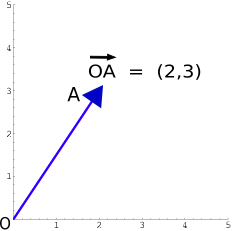
\includegraphics[width=0.25\columnwidth]{Chap07VectorSpaceRnPart1/Plane_Cartesian_vectorWikiMediaCommons.png}}%
\hspace{20pt}%
\subfloat[]{%
    \label{fig:xyP}%
	\centering
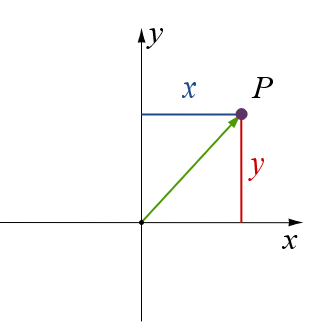
\includegraphics[width=0.25\columnwidth]{Chap07VectorSpaceRnPart1/Coord-XYWikiMediaCommons.png}}%
\caption[]{Images of the $xy$-plane with Cartesian coordinates $x$ and $y$, courtesy of the WikiMedia Commons. (a) shows a vector drawn to the \textbf{point} $(2,3)$ and labeled suggestively as a vector from the origin O to point A. (b) shows a \textbf{point} $P$ represented with coordinates $(x,y)$, also with a vector drawn to it. These are both fine interpretations of vectors. In ROB 101, points and vectors are the same thing: an ordered list of numbers.}
    \label{fig:2Dvectors}
\end{figure}




Figure~\ref{fig:2Dvectors} shows two geometric depictions of vectors in 2D, one emphasizing a vector as a directed line segment from the origin $O$ to a point $A$ located at $(2,3)$, while the second is a directed line segment from the origin $O$ to a point $P$ located at $(x,y)$. Both of these are fine interpretations of vectors. In $\real^2$, graphical depictions of vectors are relatively straightforward to understand. Figure~\ref{fig:3DSpace} illustrates so-called unit vectors along the $xyz$-axes in $\real^3$, while Fig.~\ref{fig:xyzP} shows a point in $\real^3$ with Cartesian coordinates $(x,y,z)$. These depictions of vectors and points in $\real^3$ are fairly simple, but it is not hard to give other examples in $\real^3$ that are harder to ``picture'' as a 2D-image, which is all we can show on a sheet of paper. So yes, it easy to get lost in 3D-space and if you have a hard time ``imagining'' (that is, representing visually in your head for the purpose of building intuition) objects in 3D, you are not alone. Anyone want to try $\real^{27}$, that is, 27D-space?\\

In ROB 101, points in $\real^n$ are vectors. We treat points and vectors as being different ways of representing the same mathematical object: an ordered list of numbers. Don't get hung up on the geometric aspect of vectors. In Physics, Dynamics, and Electromagnetics courses, you'll be challenged to ``imagine'' vectors in 3D. Deal with it there. For now, it is OK to think of vectors as lists of numbers that obey some basic algebraic relationships and nothing more. Besides, when dealing with a vector that has hundreds of components, what else can you do?

\begin{figure}[htb]%
\centering
\subfloat[]{%
    \label{fig:3DSpace}%
	\centering
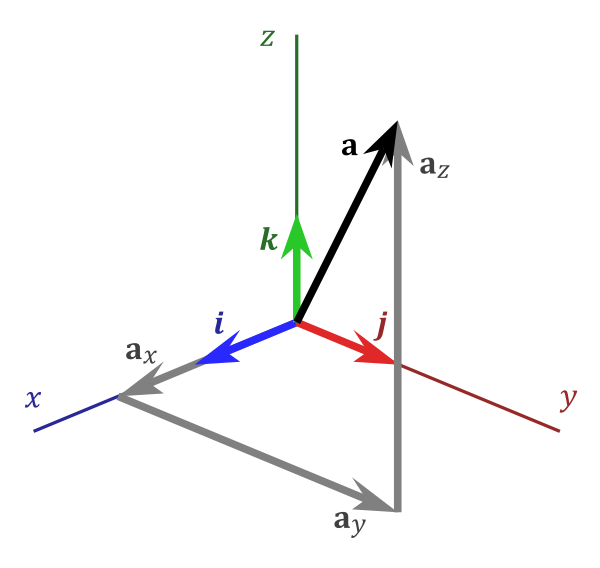
\includegraphics[width=0.35\columnwidth]{graphics/Chap07VectorSpaceRnPart1/ijk_Unit-vectors-in-Cartesian-CoordCreativeCommonsWikimediaCommons02.png}}%
\hspace{100pt}%
\subfloat[]{%
    \label{fig:xyzP}%
	\centering
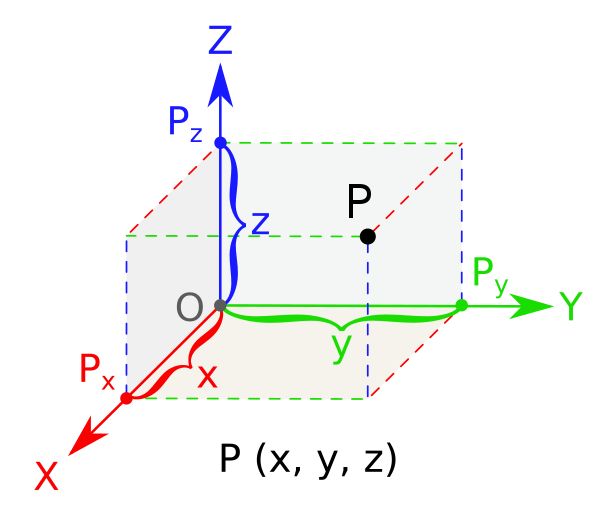
\includegraphics[width=0.35\columnwidth]{graphics/Chap07VectorSpaceRnPart1/3DSpacexyzCreativeCommons02.png}}%
\caption[]{Images of 3D space with Cartesian coordinates $x$, $y$, and $z$ using two different color schemes. (a), courtesy of WikiMedia Commons, emphasizes that the vector $a = a_x + a_y+a_z$ is the sum of three vectors lying along the $x$-axis, $y$-axis, and $z$-axis, respectively. (b), courtesy of Prof. Maani Ghaffari, emphasizes that the point $P=(x,y,z)$ has an $x$-component $P_x$, a $y$-component $P_y$, and $z$-component $P_z$. In ROB 101, points and vectors are the same thing. Moreover, we do not rely on your ability to imagine vectors in $n$-dimensional space for $n >2$.}
    \label{fig:3Dvectors}
\end{figure}

\vspace*{0.5cm}

\begin{tcolorbox}[title=\textbf{3 Special Vectors in $\real^3$}]
Figure~\ref{fig:3DSpace} defines ``unit'' vectors $\widehat{i}$, $\widehat{j}$, and $\widehat{k}$. You will see these a lot in Physics.
The more accepted mathematical notation in Linear Algebra is
$$e_1 := \begin{bmatrix} 1  \\ 0\\ 0\end{bmatrix},~e_2 := \begin{bmatrix} 0 \\ 1 \\ 0 \end{bmatrix}, ~\text{and}~ e_3 := \begin{bmatrix}0 \\ 0\\ 1 \end{bmatrix}.$$
\end{tcolorbox}


\vspace*{.5cm}

\begin{tcolorbox}[title=\textbf{Properties of Vector Addition and Scalar Times Vector Multiplication}]

 \begin{enumerate}
        \item Addition is commutative: For any $x \in \real^n$ and $y \in \real^n$, 
        $$x+y = y + x.$$
        \item Addition is associative: For any  $x \in \real^n$,  $y \in \real^n$  and $z \in \real^n$, 
        $$\left(x+y\right)+z = x+ \left( y + z \right).$$
        
        \item Scalar multiplication is associative: For any $\alpha \in \real$, $\beta \in \real$, and any $x \in \real^n$ in 
        $$\alpha \left(\beta  x \right) = \left(\alpha \beta\right) x.$$
        \item Scalar multiplication is distributive: For any $\alpha \in \real$, $\beta\in \real$ and for any $x \in \real^n$, $y\in \real^n$, 
        $$(\alpha + \beta ) x= \alpha x + \beta x ,$$
        and 
         $$\alpha \left(x + y \right) = \alpha x + \alpha y.$$
    \end{enumerate}
    
All of these properties follow from the corresponding properties for real numbers. Hence, there is no real reason to make a big deal about them. You've been adding vectors and multiplying them by constants in Julia for several weeks now!

\end{tcolorbox}



\vspace*{0.5cm}
\section{The Notion of Linear Combinations}

Sums of vectors times scalars are called linear combinations. We'll introduce the concept in two ways: first by studying what $Ax$ really means in terms of the columns of $A$ and the components of $x$, and in a second pass, a more ``pure'' or ``abstract'' definition in $\real^n$. If you enjoyed the previous 3Blue1Brown video, then I suggest you check out this one as well \url{https://www.youtube.com/watch?v=k7RM-ot2NWY}.

\subsection{Linear combinations through the lens of Ax=b}
\label{sec:LinComboExistSolutinsLensAxb}

 Let's consider $Ax=b$ and see if we truly understand the product of an $n \times m$ matrix $A$ and an $m \times 1$ column vector $x$, and then the equation $Ax=b$! We write 
 \begin{equation}
\label{eq:MatrixFromLinearIndependence_proTip}    
A=\left[\begin{array}{cccc} a_{11}& a_{12}& \cdots & a_{1m} \\
 a_{21}& a_{22}& \cdots & a_{2m}  \\
 \vdots & \vdots&  \ddots & \vdots \\
 a_{n1}& a_{n2}& \cdots & a_{nm} 
 \end{array}\right]~~\text{and}~~\left[ \begin{array}{c} x_1 \\ x_2 \\
\vdots \\ x_m   \end{array} \right]. 
 \end{equation}
Then, using our column times row method for matrix multiplication, we have
\begin{equation}
    \label{eq:bIsLinearCombinationColumnsA}
A x = \left[\begin{array}{cccc} a_{11}& a_{12}& \cdots & a_{1m} \\
 a_{21}& a_{22}& \cdots & a_{2m}  \\
 \vdots & \vdots&  \ddots & \vdots \\
 a_{n1}& a_{n2}& \cdots & a_{nm} 
 \end{array}\right] \left[ \begin{array}{c} x_1 \\ x_2 \\
\vdots \\ x_m   \end{array} \right] = \begin{bmatrix} a_{11} \\ a_{21}\\ \vdots \\ a_{n1} \end{bmatrix} {x}_1 +  \begin{bmatrix} a_{12} \\ a_{22}\\ \vdots \\ a_{n2} \end{bmatrix} {x}_2 + \cdots + \begin{bmatrix} a_{1m} \\ a_{2m}\\ \vdots \\ a_{nm} \end{bmatrix} {x}_m.
\end{equation}
If the above is not clicking for you, go back and look at our second method for matrix multiplication in Chapter~\ref{chap:MatrixMultiplication}. Note that the rows of the vector $x$ are simply its components; another way to look at is, because $x$ is $m \times 1$, its rows are $1 \times 1$.\\

The next step is to move the $x_i$ in front of the column vectors of $A$, as in
$$Ax = {x}_1 \begin{bmatrix} a_{11} \\ a_{21}\\ \vdots \\ a_{n1} \end{bmatrix}  + {x}_2  \begin{bmatrix} a_{12} \\ a_{22}\\ \vdots \\ a_{n2} \end{bmatrix}  + \cdots + {x}_m \begin{bmatrix} a_{1m} \\ a_{2m}\\ \vdots \\ a_{nm} \end{bmatrix}. $$
Because we are used to thinking of the $x_i$ as variables or unknowns, let's substitute in a ``numerical'' value, such as $\alpha_i.$ Of course, this has not changed anything, but it might look different to you,
$$A\left[ \begin{array}{c} \alpha_1 \\ \alpha_2\\
\vdots \\ \alpha_m  \end{array} \right] = \alpha_1 \begin{bmatrix} a_{11} \\ a_{21}\\ \vdots \\ a_{n1} \end{bmatrix}  + \alpha_2  \begin{bmatrix} a_{12} \\ a_{22}\\ \vdots \\ a_{n2} \end{bmatrix}  + \cdots + \alpha_m \begin{bmatrix} a_{1m} \\ a_{2m}\\ \vdots \\ a_{nm} \end{bmatrix}. $$

\begin{tcolorbox}[sharp corners, colback=green!30, colframe=green!80!blue,title=\textbf{Linear Combination of the Columns of A}]

\textbf{Definition} The following sum of scalars times vectors,
\begin{equation}
    \label{eq:EarlyDefLinearCombination}
    \alpha_1 \begin{bmatrix} a_{11} \\ a_{21}\\ \vdots \\ a_{n1} \end{bmatrix}  + \alpha_2  \begin{bmatrix} a_{12} \\ a_{22}\\ \vdots \\ a_{n2} \end{bmatrix}  + \cdots + \alpha_m \begin{bmatrix} a_{1m} \\ a_{2m}\\ \vdots \\ a_{nm} \end{bmatrix},
\end{equation}
is called a \textbf{linear combination} of the columns of $A$. When we set $A\alpha = b$, and turn it around as $b =A \alpha$, we arrive at an important \textbf{Fact:} a vector $\alpha \in \real^m$ is a solution to $Ax=b$ (that is, $A \alpha = b$) if, and only if
\begin{equation}
    \label{eq:EarlyDefLinearCombinationWithb}
   b= \alpha_1 \begin{bmatrix} a_{11} \\ a_{21}\\ \vdots \\ a_{n1} \end{bmatrix}  + \alpha_2  \begin{bmatrix} a_{12} \\ a_{22}\\ \vdots \\ a_{n2} \end{bmatrix}  + \cdots + \alpha_m \begin{bmatrix} a_{1m} \\ a_{2m}\\ \vdots \\ a_{nm} \end{bmatrix},
\end{equation}
that is, $b$ can be expressed as a linear combination of the columns of $A$.
We will revisit this later, but \eqref{eq:EarlyDefLinearCombinationWithb} is a primary motivation for introducing the notion of linear combinations.
\end{tcolorbox}

\subsection{Linear Combinations in $\real^n$}

\begin{tcolorbox}[title=\textbf{Linear Combination}]
A vector $v\in \real^n$ is a \textbf{linear combination of} $\{u_1, u_2, \ldots, u_m\} \subset \real^n$ if there exist real numbers $\alpha_1, \alpha_2, \ldots, \alpha_m$ such that
\begin{equation}
    \label{eq:DefLinearCombinationRn}
    v = \alpha_1 u_1 + \alpha_2 u_2 + \cdots + \alpha_m u_m.
\end{equation}

\end{tcolorbox}

\vspace*{0.5cm}

\begin{example}
\label{ex:LinearComboA1}
Because 
$$\underbrace{\begin{bmatrix} -3 \\  -5 \\ -7\end{bmatrix}}_{v}=2\underbrace{\begin{bmatrix} 3 \\  2 \\ 1\end{bmatrix}}_{u_1} - 9 \underbrace{ \begin{bmatrix} 1 \\  1 \\ 1\end{bmatrix}}_{u_2},$$
we have that $v$ is a linear combination of $\{u_1, u_2\}$.
\end{example}

When you are given the coefficients, it is easy to observe that a given vector is a linear combination of other vectors. But when you have to check if such coefficients exist or do not exist, then it's just a wee bit more challenging!
\vspace*{0.5cm}

\begin{example}
\label{ex:LinearComboA2}
Is the vector $v= \begin{bmatrix} 4 \\  4 \\ 4\end{bmatrix}$ a linear combination of 
$$u_1=\left[\begin{array}{r} 3 \\ 1\\ -1  \end{array} \right]~~\text{and}~~u_2=\left[\begin{array}{r} 2 \\ -2\\ 1  \end{array} \right]? $$
\end{example}

\textbf{Solution:} The vector $v$ is a linear combination of the vectors $u_1$ and $u_2$ if, and only if, there exist real numbers $\alpha_1$ and $\alpha_2$ such that
\begin{equation}
\label{eq:LinearCombination}
   \alpha_1 u_1 + \alpha_2 u_2 = v. 
\end{equation} 
What we have done here is apply\footnote{In the beginning, many of us are confused about how to go about solving a problem. Sound advice is to start with the definitions at your disposal. Then try to turn the definition into a set of equations to be solved.} \textbf{the definition of a linear combination.}
So, we write down the linear equations corresponding to \eqref{eq:LinearCombination}, namely
\begin{equation}
\label{eq:CheckLinearCombinationEquations}
\begin{aligned}
    \alpha_1 \left[ \begin{array}{r} 3 \\ 1 \\ -1   \end{array} \right] + \alpha_2 \left[ \begin{array}{r} 2 \\ -2 \\ 1   \end{array} \right] &= \left[ \begin{array}{r} 4 \\ 4 \\ 4   \end{array} \right]\\
   & \Updownarrow \\
    \left[ \begin{array}{rr} 3 & 2\\ 1  & -2\\ -1  & 1 \end{array} \right]  \left[ \begin{array}{r} \alpha_1 \\ \alpha_2 \end{array} \right] &= \left[ \begin{array}{r} 4 \\ 4 \\ 4   \end{array} \right]
\end{aligned}
\end{equation}
and see if we can find a solution for the \textbf{unknowns} $\alpha_1$ and $\alpha_2$! What makes this look hard is that we have a non-square (rectangular) system of linear equations, namely, three equations and two unknowns.\\

What are the three equations? They may look more familiar to you if we write them out like this,
\begin{align*}
   3 \alpha_1 + 2 \alpha_2 &=4 \\
   \alpha_1 - 2 \alpha_2 &= 4\\
   -\alpha_1 + \alpha_2 &= 4.
\end{align*}

A systematic way to approach such problems is to observe that if $\alpha_1$ and $\alpha_2$ are to simultaneously satisfy all three equations, then they must necessarily satisfy any two of them. Moreover, if you find that the solution to the resulting square system of two equations and two unknowns is unique, then two things are possible:
\begin{itemize}
    \item the solution of the smaller square system of equations also satisfies the equation(s) you did not use, giving you a solution to the full set of equations, or
    \item the solution of the smaller square system of equations does not satisfy the equation(s) you did not use, telling you that the full set of equations is inconsistent and does not have a solution.
\end{itemize}

In our case, if we remove the last equation, we have 
\begin{equation}
\label{eq:CheckLinearCombinationEquationsKeepTwo}
\begin{aligned}
       \left[ \begin{array}{rr} 3 & 2\\ 1  & -2 \end{array} \right]  \left[ \begin{array}{r} \alpha_1 \\ \alpha_2 \end{array} \right] &= \left[ \begin{array}{r} 4 \\ 4   \end{array} \right],
\end{aligned}
\end{equation}
and we observe that the matrix multiplying the vector of unknowns has determinant $-8$, and thus \eqref{eq:CheckLinearCombinationEquationsKeepTwo} has a unique solution. A bit of matrix magic with our formula for a $2 \times 2$ inverse gives
 $$\alpha_1=2~~\text{and}~\alpha_2=-1. $$
 Do these values satisfy the equation we did not use, namely, the last row of \eqref{eq:CheckLinearCombinationEquationsKeepTwo},
 $$\left[ \begin{array}{rr} -1  & 1 \end{array} \right]  \left[ \begin{array}{r} \alpha_1 \\ \alpha_2 \end{array} \right] = \left[ \begin{array}{r} 4\end{array} \right]? $$
Clearly not, because $-1 \alpha_1 + \alpha_2 = -3 \neq 4,$ and
\textbf{hence, $v$ is NOT a linear combination of $u_1$ and $u_2$.} 

\vspace*{0.5cm}

\begin{tcolorbox}
The key point is that $\alpha_1$ and $\alpha_2$ must satisfy all three equations in \eqref{eq:CheckLinearCombinationEquations}. It does not matter in what order we use the equations when seeking a solution. To illustrate that, we'll first solve the last two equations, 
\begin{align*}
     \alpha_1 - 2 \alpha_2 &= 4 \\
 -\alpha_1 + \alpha_2 &= 4,
\end{align*}
which yields, $\alpha_1=-12$ and $\alpha_2=-8$. We then check if these values satisfy the first equation
$$ 3\alpha_1 +2 \alpha_2 = 4 \iff -36  - 16 = 4 \iff -52= 4,$$
which is false, and therefore, $v$ is NOT a linear combination of $u_1$ and $u_2$.
\end{tcolorbox}

\vspace*{.5cm} 

\textbf{Rework the problem:} Let's keep $u_1$ and $u_2$ as given and change $v$ to
$$\tilde{v}=  \left[ \begin{array}{r} 0 \\ -8 \\ 5   \end{array} \right].$$
Applying the above strategy to the equations
\begin{align*}
   3 \alpha_1 + 2 \alpha_2 &=0\\
   \alpha_1 - 2 \alpha_2 &= -8\\
   -\alpha_1 + \alpha_2 &= 5
\end{align*}
yields $\alpha_1=-2$ and $\alpha_2=3$, as you can verify by direct substitution. \textbf{Hence, $\tilde{v}$ is a linear combination of $u_1$ and $u_2$.} \Qed

\vspace*{0.5cm}

\textbf{Remark:} Checking whether a given vector can be written as a linear combination of other vectors always comes down to solving a system of linear equations. If that system is square with a non-zero determinant, then solving the system of equations is cake. Otherwise, solving the equations by hand is mostly painful. \textbf{We will need to develop a better way to check if a vector is, or is not, a linear combination of other vectors!}

\section{Existence of Solutions to Ax=b}
\label{sec:UniquenessSolutions}

Because it is so important, we now revisit the relation of linear combinations to the existence of solutions to systems of linear equations. We want to make sure you did NOT miss something important when reading Chapter~\ref{sec:LinComboExistSolutinsLensAxb}. If you are confident of your knowledge, then feel free to move on to the next section. Otherwise, please read on!\\

Let $A$ be an $n \times m$ matrix, not necessarily square, as in \eqref{eq:ColumnsOfMatrixVectorsRn}. Recall that columns of $A$ and vectors in $\real^n$ are the same thing. We write out $Ax=b$ is all its glory, 
\begin{equation}
\label{eq:ExistenceSolutionsNonsquare}    
 \underbrace{\left[\begin{array}{cccc} a_{11}& a_{12}& \cdots & a_{1m} \\
 a_{21}& a_{22}& \cdots & a_{2m}  \\
 \vdots & \vdots&  \ddots & \vdots \\
 a_{n1}& a_{n2}& \cdots & a_{nm} 
 \end{array}\right] }_{A} \underbrace{\left[ \begin{array}{c} x_1 \\ x_2 \\
\vdots \\ x_m   \end{array} \right]}_{x} = \underbrace{\left[ \begin{array}{c} b_1 \\ b_2 \\ \vdots \\ b_n  \end{array} \right]}_{b}.
\end{equation}

\vspace*{.5cm}
\begin{tcolorbox}[sharp corners, colback=green!30, colframe=green!80!blue, title=\textbf{\large Existence of Solutions}] 
The equation $Ax=b$ has a solution if, and only if, $b$ can be written as a linear combination of the columns of $A$.
\end{tcolorbox}

\vspace{0.5cm}
\begin{tcolorbox}%[title=\textbf{Why it is true}]
\textbf{The following is more or less a proof:} Suppose that $\bar{x}$ satisfies $A \bar{x} =b$, which is the same thing as saying $\bar{x}$ is a solution of $Ax=b$. Then, doing the indicated multiplication of $A \bar{x}$ via our now favorite method, the columns of $A$ times the rows of the vector $\bar{x}$, which are its scalar entries $\bar{x}_i$, yields
\begin{equation}
    \label{eq:bIsLinearCombinationColumnsA02}
\begin{bmatrix} a_{11} \\ a_{21}\\ \vdots \\ a_{n1} \end{bmatrix} \bar{x}_1 +  \begin{bmatrix} a_{12} \\ a_{22}\\ \vdots \\ a_{n2} \end{bmatrix} \bar{x}_2 + \cdots + \begin{bmatrix} a_{1m} \\ a_{2m}\\ \vdots \\ a_{nm} \end{bmatrix} \bar{x}_m = \begin{bmatrix} b_1 \\ b_2\\ \vdots \\ b_m \end{bmatrix}
\end{equation}
Exchanging the two sides of the equal sign and moving the scalars $\bar{x}_i$ to the front of the vectors give
\begin{equation}
    \label{eq:bIsLinearCombinationColumnsAflipped}
 \begin{bmatrix} b_1 \\ b_2\\ \vdots \\ b_m \end{bmatrix} = \bar{x}_1 \begin{bmatrix} a_{11} \\ a_{21}\\ \vdots \\ a_{n1} \end{bmatrix}+ \bar{x}_2 \begin{bmatrix} a_{12} \\ a_{22}\\ \vdots \\ a_{n2} \end{bmatrix} + \cdots + \bar{x}_m \begin{bmatrix} a_{1m} \\ a_{2m}\\ \vdots \\ a_{nm} \end{bmatrix};
\end{equation}
in other words, $b$ is a linear combination of the columns of $A$. The other way around works as well: if we manage to write 
$$b = c_1  a_1^{\rm col} + c_2 a_2^{\rm col} + \cdots c_m a_m^{\rm col}$$
for some real numbers $c_i \in \real$, then $\bar{x}=\begin{bmatrix} c_1 & c_2 & \cdots & c_m \end{bmatrix}^\top$ satisfies $A \bar{x}=b$, and hence it is a solution to $Ax=b$. \\

Recall that $a_j^{\rm col}:=\begin{bmatrix} a_{ij} & a_{2j}  & \cdots & a_{nj} \end{bmatrix}^\top, 1 \le j \le m.$
\end{tcolorbox}

A weakness of the above result is that we do not yet have an effective means for checking whether or not a given vector is a linear combination of a specified set of vectors. We will solve this problem too, a little bit later in the Chapter. All we have done so far is indicate that the concept of a linear combination is related to the existence of a solution to a corresponding system of linear equations. \textbf{The result is mainly conceptual in that we have not yet provided a practical way to check this in code. That will come, though! Long Live the LU Factorization!}


\section{Linear Independence of a Set of Vectors}

\subsection{Preamble}
The concept of \textit{linear independence}, or its logical opposite, the concept of \textit{linear dependence}, is one of the most important ideas in all of linear algebra. In the beginning, most of us struggle with two things: (1) why is the property of linear independence so important; and (2), how do you test for it? In this section, we highlight the importance of linear independence of vectors by relating it to uniqueness of solutions to $\mathbf{Ax=0}$ and eventually, to uniqueness of solutions to $\mathbf{Ax=b}$. We'll also show that our friend, the LU Factorization, makes testing for linear independence very straightforward. 

\subsection{Linear Independence through the Lens of Ax=0}

Let $A$ be an $n \times m$ matrix. We say that $x\in \real^m$ is a \textbf{nontrivial solution} to $Ax=0_{n \times 1}$ if
\begin{itemize}
    \item $Ax=0_{n \times 1}$ ($x$ is a solution), and 
    \item $x\neq0_{m \times 1} $ ($x$ is not the zero vector in $\real^m)$. 
\end{itemize}
Because $x=0$ is always a solution to $Ax=0$, for it to be the \textbf{unique solution}, there must not be a non-trivial solution to $Ax=0.$\\

Why are we making such a big deal about this? Because uniqueness is a desirable property and we want to learn how to check for it even in the case of rectangular systems of equations\footnote{Recall, when $A$ is square, uniqueness is equivalent to $\det(A)\neq 0$.}. Our immediate goal is to see what this means in terms of the columns of $A$, just as we did when introducing the notion of a linear combination. \\

To see what it means to have ``non-trivial solutions'' to $Ax=0_{n \times 1}$, once again, we replace $x \in \real^m$ by a vector $\alpha \in \real^m$ and write
 \begin{equation}
\label{eq:MatrixFromLinearIndependence_proTipB}    
A=\left[\begin{array}{cccc} a_{11}& a_{12}& \cdots & a_{1m} \\
 a_{21}& a_{22}& \cdots & a_{2m}  \\
 \vdots & \vdots&  \ddots & \vdots \\
 a_{n1}& a_{n2}& \cdots & a_{nm} 
 \end{array}\right]~~\text{and}~~\alpha =\left[ \begin{array}{c} \alpha_1 \\ \alpha_2 \\
\vdots \\ \alpha_m   \end{array} \right]. 
 \end{equation}
Then, using our column times row method for matrix multiplication, and re-arranging terms a bit as we did in Chapter~\ref{sec:LinComboExistSolutinsLensAxb},
\begin{equation}
    \label{eq:LinearIndepColumnsA01}
    \begin{aligned}
A \alpha &= \left[\begin{array}{cccc} a_{11}& a_{12}& \cdots & a_{1m} \\
 a_{21}& a_{22}& \cdots & a_{2m}  \\
 \vdots & \vdots&  \ddots & \vdots \\
 a_{n1}& a_{n2}& \cdots & a_{nm} 
 \end{array}\right] \left[ \begin{array}{c} \alpha_1 \\ \alpha_2\\
\vdots \\ \alpha_m  \end{array} \right] \\
& = \alpha_1 \begin{bmatrix} a_{11} \\ a_{21}\\ \vdots \\ a_{n1} \end{bmatrix}  + \alpha_2  \begin{bmatrix} a_{12} \\ a_{22}\\ \vdots \\ a_{n2} \end{bmatrix}  + \cdots + \alpha_m \begin{bmatrix} a_{1m} \\ a_{2m}\\ \vdots \\ a_{nm} \end{bmatrix}.
    \end{aligned}
\end{equation}
Hence, $A\alpha = 0_{n \times 1}$ if, and only if, 
\begin{equation}
    \label{eq:LinearIndepColumnsA02}
    \begin{aligned}
\alpha_1 \begin{bmatrix} a_{11} \\ a_{21}\\ \vdots \\ a_{n1} \end{bmatrix}  + \alpha_2  \begin{bmatrix} a_{12} \\ a_{22}\\ \vdots \\ a_{n2} \end{bmatrix}  + \cdots + \alpha_m \begin{bmatrix} a_{1m} \\ a_{2m}\\ \vdots \\ a_{nm} \end{bmatrix} & = \begin{bmatrix} 0 \\ 0\\ \vdots \\ 0 \end{bmatrix}_{n \times 1}.
    \end{aligned}
\end{equation}
Our takeaway is, $\alpha = 0_{m \times 1}$ is the unique solution to $A\alpha=0$ if, and only if, the only way we can add up the columns of $A$ and obtain the zero vector in $\real^n$ is with 
$$\alpha_1=0, \alpha_2=0, \ldots, \alpha_m=0. $$
Or equivalently, $A\alpha = 0$ has a non-trivial solution $\alpha \neq 0_{m \times 1}$, if, and only if, there exists real numbers $\alpha_1, \alpha_2, \ldots, \alpha_m$, \textbf{NOT ALL ZERO}, such that \eqref{eq:LinearIndepColumnsA02} is satisfied.

\subsection{Linear Independence in $\real^n$ (and why theory matters)}

The definition of linear independence of an ``abstract'' set of vectors in $\real^n$ is 100\% motivated by the study above on the uniqueness of solutions to $Ax=0.$ Of course, vectors in $\real^n$ are columns of $n \times m$ matrices, so who's to say what is abstract and what is not!

\vspace*{0.5cm}

\begin{tcolorbox}[sharp corners, colback=green!30, colframe=green!80!blue, title=\textbf{Linear Independence of a Set of Vectors}]
 The set of vectors $\{v_1, v_2, ..., v_m \} \subset \real^n$ is \textbf{linearly dependent} if there exist real numbers $\alpha_1, \alpha_2, \ldots, \alpha_m$ \textbf{NOT ALL ZERO} yielding a linear combination of vectors that adds up to the zero vector,
\begin{equation}
    \alpha_1 v_1 + \alpha_2 v_2 + \ldots + \alpha_m v_m =0_{n \times 1}.
\end{equation}

On the other hand, the vectors $\{v_1, v_2, ..., v_m \}$ are \textbf{linearly independent} if the \textbf{only} real numbers $\alpha_1, \alpha_2, \ldots, \alpha_m$ yielding a linear combination of vectors that adds up to the zero vector,
\begin{equation}
    \alpha_1 v_1 + \alpha_2 v_2 + \ldots + \alpha_m v_m =0_{n \times 1},
    \end{equation}
are $\boldsymbol{\alpha}_1= \mathbf{0}, \boldsymbol{\alpha}_2=\mathbf{0}, \ldots, \boldsymbol{\alpha}_m=\mathbf{0}.$\\

\textbf{Concise Definition of Linear Independence:} 
$$\alpha_1 v_1 + \alpha_2 v_2 + \ldots + \alpha_m v_m =0_{n \times 1}  \iff \begin{bmatrix} \alpha_1 \\ \alpha_2 \\ \vdots \\ \alpha_m \end{bmatrix} = \begin{bmatrix} 0 \\ 0 \\ \vdots \\ 0 \end{bmatrix}= 0_{m \times 1}.$$
\end{tcolorbox}

\vspace*{.5cm}
\begin{example} 
\label{ex:LinearIndep02} By applying the definition, determine if the set of vectors
$$v_1 = \left[ \begin{array}{r} \sqrt{2} \\0\\  0  \end{array} \right]  , v_2 = \left[ \begin{array}{r}  4 \\ 7  \\0  \end{array} \right], v_3 = \left[ \begin{array}{r} 3 \\ 1 \\ -1   \end{array} \right] $$
is linearly independent or dependent.
\end{example}

\textbf{Solution:} We form the linear combination and do the indicated multiplications and additions
\begin{equation}
\label{eq:LinearIndependenceExample02}
    \alpha_1 v_1 + \alpha_2 v_2 + \alpha_3 v_3 = 
    \alpha_1 \left[ \begin{array}{r} \sqrt{2} \\0\\ 0  \end{array} \right] 
+ \alpha_2 \left[ \begin{array}{r}  4 \\ 7 \\ 0  \end{array} \right] 
+ \alpha_3 \left[ \begin{array}{r} 3 \\ 1 \\ -1   \end{array} \right]  = \left[ \begin{array}{r}  \sqrt{2}\  \alpha_1  + 4\ \alpha_2 + 3\ \alpha_3\\7 \ \alpha_2 + \alpha_3\\  -1\ \alpha_3 \end{array} \right].
\end{equation}
Setting the right hand side of \eqref{eq:LinearIndependenceExample02} to the zero vector yields
\begin{equation}
\label{eq:LinearIndependenceExample02b}
   \left[ \begin{array}{r}  \sqrt{2}\  \alpha_1  + 4\ \alpha_2 + 3\ \alpha_3\\7 \ \alpha_2 + \alpha_3\\  -1\ \alpha_3 \end{array} \right] = \left[ \begin{array}{r} 0 \\ 0 \\ 0   \end{array} \right].
\end{equation}
This is one of our friendly triangular systems of linear equations which we can solve via back substitution. We see immediately that the only solution to the bottom equation is $\alpha_3=0$, the only solution to the middle equation is then $\alpha_2 = 0$, and finally, the only solution to the top equation is $\alpha_1=0$. Hence, the only solution to 
$$ \alpha_1 v_1 + \alpha_2 v_2 + \alpha_3 v_3 =0 $$
is $\alpha_1=0$, $\alpha_2 = 0$, and $\alpha_3=0$, and hence the set of vectors  $ \{v_1, v_2, v_3 \} $ is linearly independent.\\

The above analysis becomes even more clear when we write \eqref{eq:LinearIndependenceExample02b} as
\begin{equation}
\label{eq:LinearIndependenceExample02c}
   \left[ \begin{array}{ccr}  \sqrt{2} &  4 &  3 \\ 0 & 7  & 1 \\ 0 & 0 & -1  \end{array} \right]\left[ \begin{array}{r} \alpha_1 \\ \alpha_2 \\ \alpha_3   \end{array} \right] = \left[ \begin{array}{r} 0 \\ 0 \\ 0   \end{array} \right] .
\end{equation}
We see that the matrix is square with a non-zero determinant, and hence we know it has a unique solution. 
 \Qed \\
 
 \vspace{.5cm}

\begin{example} 
\label{ex:LinearIndep00} By applying the definition, determine  if the set of vectors $$ v_1 = \left[ \begin{array}{r} 1 \\2\\  3 \end{array} \right]  , v_2 = \left[ \begin{array}{r}  1 \\ -2  \\-4  \end{array} \right] $$
is linearly independent or dependent.
\end{example}

\textbf{Solution:} We seek to determine if there are non-zero coefficients $\alpha_1$ and $\alpha_2$ resulting in a linear combination that forms the zero vector in $\real^3$,
\begin{equation}
\label{eq:LinearIndependenceExample00a}
    \alpha_1 v_1 + \alpha_2 v_2  = 
    \alpha_1 \left[ \begin{array}{r} 1 \\2\\  3  \end{array} \right] 
+ \alpha_2 \left[ \begin{array}{r}  1 \\ -2  \\-4  \end{array} \right] =  \left[ \begin{array}{r} \alpha_1 + \alpha_2\\ 2 \alpha_1 -2  \alpha_2 \\ 3 \alpha_1 -4 \alpha_2 \end{array} \right] = \left[ \begin{array}{r} 0 \\ 0 \\0\end{array} \right].
\end{equation}
We observe that we have three equations in two unknowns and no obvious triangular structure to help us! What do we do? Well, if we can take any two of the three equations and show that the only solution is the trivial solution,  $\alpha_1=0$ and $\alpha_2=0$, then we are done, because the trivial solution will always satisfy the remaining equation. Please check this reasoning out for yourself.\\

We arbitrarily group the equations into the first two equations and then the last equation, as follows 
\begin{align}
\label{eq:LinearIndependenceExample00b1}
    \alpha_1 \left[ \begin{array}{r} 1 \\2\\ \end{array} \right] 
+ \alpha_2 \left[ \begin{array}{r}  1 \\ -2   \end{array} \right] &= \left[ \begin{array}{r} 0 \\ 0 \end{array} \right] \\
\label{eq:LinearIndependenceExample00b2}
\alpha_1 \left[ \begin{array}{r} 3 \end{array} \right] + \alpha_2 \left[ \begin{array}{r} -4\end{array} \right] &= 0.
\end{align}

We can rewrite \eqref{eq:LinearIndependenceExample00b1} in the form $A \alpha=b$
\begin{equation}
\label{eq:LinearIndependenceExample00c1}
   \underbrace{\left[ \begin{array}{rr} 1 & 1\\2 & -2 \end{array} \right]}_{A} 
\underbrace{\left[ \begin{array}{c} \alpha_1 \\ \alpha_2 \end{array} \right]}_{\alpha} =  \underbrace{ \left[ \begin{array}{r} 0 \\ 0 \end{array} \right]}_{b}.
\end{equation}
We note that $\det(A) = (1)(-2)-(1)(2) = -4 \neq 0$, and hence \eqref{eq:LinearIndependenceExample00c1} has a unique solution. Because $\alpha_1=0$ and $\alpha_2=0$ is a solution and the solution is unique, we know that there cannot exist a different set of non-zero  $\alpha_1$ and $\alpha_2$ that also solve the equation. We, therefore, conclude that the vectors $\{v_1, v_2\}$ are linearly independent. \\

\textbf{Remark:} Let's step back and see what is going on here. We have three equations and two unknowns. The trivial  solution is always a solution to the full set of equations. We wonder if there is any other solution. If we make a choice of two of the equations, so that we have a more manageable square system of equations, and then find that those two equations constrain the solution to being the trivial solution, we are done! (Why, because the trivial solution will automatically satisfy the remaining equation and it is then the only solution that satisfies all three equations.)
 \Qed\\
 
 
That was a lot of work! It does not seem like it will scale to bigger sets of vectors.  We'll do one more example to convince you that we are in dire need of a \textbf{Pro Tip!}

\vspace*{0.5cm}

\begin{example} 
\label{ex:LinearIndep01} By applying the definition, determine  if the vectors 
$$v_1 = \left[ \begin{array}{r} 1 \\2\\  3 \\1  \end{array} \right]  , v_2 = \left[ \begin{array}{r}  0 \\ -2  \\4 \\ 5  \end{array} \right], v_3 = \left[ \begin{array}{r} 2 \\ 6 \\ 2  \\ -3 \end{array} \right] $$
are linearly independent or dependent.
\end{example}

\textbf{Solution:} We form the linear combination and set it equal to zero,
\begin{equation}
\label{eq:LinearIndependenceExample01}
    \alpha_1 v_1 + \alpha_2 v_2 + \alpha_3 v_3 = 
    \alpha_1 \left[ \begin{array}{r} 1 \\2\\  3 \\1  \end{array} \right] 
+ \alpha_2 \left[ \begin{array}{r}  0 \\ -2  \\4 \\ 5  \end{array} \right]
+ \alpha_3 \left[ \begin{array}{r} 2 \\ 6 \\ 2  \\ -3 \end{array} \right]  = \left[ \begin{array}{r} \alpha_1  +2\ \alpha_3 \\ 2 \alpha_1 -2 \alpha_2 + 6 \alpha_3\\ 3 \alpha_1+ 4 \alpha_2 +  2 \alpha_3  \\ \alpha_1+ 5 \alpha_2 -3 \alpha_3 \end{array} \right] = \left[ \begin{array}{r}  0 \\ 0 \\0 \\0  \end{array} \right].
\end{equation}
\textbf{We must check whether or not there are \textit{non-trivial} solutions to} \eqref{eq:LinearIndependenceExample01}, where non-trivial means at least one of the coefficients $\alpha_1$,  $\alpha_2$, or  $\alpha_3$ is non-zero.\\ 

We observe that we have four equations in three unknowns. Similar to Example~\ref{ex:LinearIndep00}, we could select any three of the four equations, solve those three, and then see if that solution is compatible with the remaining equation. Once again, this will be a lot of work. We'll save ourselves the effort and let you verify that $\alpha_1=2, \alpha_2=-1, \alpha_3 = -1$ is a non-trivial solution to \eqref{eq:LinearIndependenceExample01} and hence the vectors $v_1, v_2, v_3$ are linearly dependent. \textbf{Where is that Pro Tip?} \Qed\\



% % The method in Example~\ref{ex:LinearIndep02} is completely general, and we summarize it in the following. 
% \vspace*{0.5cm}
% \begin{tcolorbox}[sharp corners, colback=green!30, colframe=green!80!blue, title=\textbf{\large Relating Linear Independence of Vectors to a System of Linear Equations}]
% Consider the vector space $\real^n$ and a set of vectors 
% $$\left\{v_1=\begin{bmatrix} a_{11} \\ a_{21}\\ \vdots \\ a_{n1} \end{bmatrix}, v_2=\begin{bmatrix} a_{12} \\ a_{22}\\ \vdots \\ a_{n2} \end{bmatrix}, ..., v_m=\begin{bmatrix} a_{1m} \\ a_{2m}\\ \vdots \\ a_{nm} \end{bmatrix} \right\}$$ 
% in $\real^n$. \textbf{The following statements are equivalent:} 
% \begin{enumerate}
% \renewcommand{\labelenumi}{(\alph{enumi})}
% \setlength{\itemsep}{.2cm}
%     \item $\{v_1, v_2, ..., v_m \}$ is a linearly independent set of vectors
%     \item The only solution to 
% $$
%     \alpha_1 v_1 + \alpha_2 v_2 + \ldots + \alpha_m v_m =0
% $$
% is the trivial solution $\alpha_1=0, \alpha_2 = 0, \ldots, \alpha_m=0.$

% \item The only solution to the set of linear equations
% \begin{equation}
% \label{eq:MatrixFromLinearIndependence}    
%  \underbrace{\left[\begin{array}{cccc} a_{11}& a_{12}& \cdots & a_{1m} \\
%  a_{21}& a_{22}& \cdots & a_{2m}  \\
%  \vdots & \vdots&  \ddots & \vdots \\
%  a_{n1}& a_{n2}& \cdots & a_{nm} 
%  \end{array}\right] }_{A} \underbrace{\left[ \begin{array}{c} \alpha_1 \\ \alpha_2 \\
% \vdots \\ \alpha_m   \end{array} \right]}_{\alpha} = \underbrace{\left[ \begin{array}{c} 0 \\ 0 \\ \vdots \\ 0  \end{array} \right]}_{0}
% \end{equation}
% is the trivial solution, $\alpha=0$.
% \item The only solution to the set of linear equations
% \begin{equation}
% \label{eq:MatrixFromLinearIndependenceWithx}    
%  \underbrace{\left[\begin{array}{cccc} a_{11}& a_{12}& \cdots & a_{1m} \\
%  a_{21}& a_{22}& \cdots & a_{2m}  \\
%  \vdots & \vdots&  \ddots & \vdots \\
%  a_{n1}& a_{n2}& \cdots & a_{nm} 
%  \end{array}\right] }_{A} \underbrace{\left[ \begin{array}{c} x_1 \\ x_2 \\
% \vdots \\ x_m   \end{array} \right]}_{x} = \underbrace{\left[ \begin{array}{c} 0 \\ 0 \\ \vdots \\ 0  \end{array} \right]}_{0}
% \end{equation}
% is the trivial solution, $x=0$.
% \item $x = 0$ (the zero vector) is the unique solution to $A x = 0.$

% \item The columns of the matrix $A$ are linearly independent.
% \end{enumerate}

%  \textbf{Remark:} This is probably way more than you needed to see. But, 

% % \textbf{Remark:} We have two more things to do: relate linear independence to uniqueness of solutions to $Ax=b$ and show how LU Factorization makes it trivial to check the condition \eqref{eq:MatrixFromLinearIndependence}, or equivalently, the condition \eqref{eq:MatrixFromLinearIndependenceWithx}.
% \end{tcolorbox}
\subsection{A Pro Tip for Checking Linear Independence}
\label{sec:proTipLinearIndependence}

\begin{tcolorbox}[sharp corners, colback=green!30, colframe=green!80!blue,
title=\textbf{Pro-tip! Linear Independence in a Nutshell}]
Consider the vectors in $\real^n$,
$$\left\{v_1=\begin{bmatrix} a_{11} \\ a_{21}\\ \vdots \\ a_{n1} \end{bmatrix},  v_2=\begin{bmatrix} a_{12} \\ a_{22}\\ \vdots \\ a_{n2} \end{bmatrix}, ...,  v_m=\begin{bmatrix} a_{1m} \\ a_{2m}\\ \vdots \\ a_{nm} \end{bmatrix} \right\},$$ 
and use them as the columns of a matrix that we call $A$,
\begin{equation}
\label{eq:MatrixFromLinearIndependence_proTipC}    
A=\left[\begin{array}{cccc} a_{11}& a_{12}& \cdots & a_{1m} \\
 a_{21}& a_{22}& \cdots & a_{2m}  \\
 \vdots & \vdots&  \ddots & \vdots \\
 a_{n1}& a_{n2}& \cdots & a_{nm} 
 \end{array}\right].
 \end{equation}
 The following statements are equivalent:
 \begin{itemize}
     \item  The set of vectors $ \{v_1, v_2, \ldots, v_m \} $ is linearly independent.
     \item The $m \times m$ matrix $A^\top \cdot A$ is invertible. 
     \item $\det(A^\top \cdot A) \neq 0$.
     \item For any LU Factorization $P \cdot (A^\top \cdot A) = L \cdot U$  of $A^\top A$, the $m \times m$ upper triangular matrix $U$ has no zeros on its diagonal.
 \end{itemize}
 
We'll prove the Pro Tip shortly. For now, we'll focus on how it makes our lives so much easier in terms of checking linear independence.
\end{tcolorbox}

\vspace*{.1cm}

\begin{example} 
\label{ex:LinearIndep04} We apply the Pro Tip to Example~\ref{ex:LinearIndep02}
\end{example}

\textbf{Solution:} We use the vectors $ v_1 = \left[ \begin{array}{r} 1 \\2\\  3 \end{array} \right]~~\text{and}~~ v_2 = \left[ \begin{array}{r}  1 \\ -2  \\-4  \end{array} \right] $ 
as the columns of a matrix $ A:=[ v_1 ~~v_2]$, so that 
$$A=\left[ \begin{array}{rr} 1 & 1\\2 & -2\\  3 & -4\end{array} \right]. $$
We compute that
$$
A^\top \cdot A = \left[
\begin{array}{rr}
14.0 & -15.0 \\
-15.0 & 21.0 \\
\end{array}
\right].
$$
Because it is $2\times 2$, we can compute its determinant easily and obtain 
$$ \det(A^\top \cdot A)=69.0 \neq 0,$$
and hence the vectors $\{ v_1, v_2\}$ are linearly independent. 
\Qed
\vspace*{.5cm}

\begin{example} 
\label{ex:LinearIndep05} We apply the Pro Tip to Example~\ref{ex:LinearIndep01}. 
\end{example}

\textbf{Solution:} We use the vectors $$v_1 = \left[ \begin{array}{r} 1 \\2\\  3 \\1  \end{array} \right]  , v_2 = \left[ \begin{array}{r}  0 \\ -2  \\4 \\ 5  \end{array} \right], v_3 = \left[ \begin{array}{r} 2 \\ 6 \\ 2  \\ -3 \end{array} \right] $$
and form the matrix
$$A:= \left[ \begin{array}{rrr} 1  & 0 & 2\\2 & -2 & 6\\  3 & 4 & 2 \\1 & 5 & -3  \end{array} \right]. $$
We go to Julia and compute that
$$ A^\top \cdot A =
\left[
\begin{array}{rrr}
15.0 & 13.0 & 17.0 \\
13.0 & 45.0 & -19.0 \\
17.0 & -19.0 & 53.0 \\
\end{array}
\right],
$$
and that its LU Factorization is $P\cdot \left( A^\top \cdot A \right) = L \cdot U$, where
$$P = \left[
\begin{array}{ccc}
0.0 & 0.0 & 1.0 \\
0.0 & 1.0 & 0.0 \\
1.0 & 0.0 & 0.0 \\
\end{array}
\right],~~ L=
\left[
\begin{array}{ccc}
1.0 & 0.0 & 0.0 \\
0.8 & 1.0 & 0.0 \\
0.9 & 0.5 & 1.0 \\
\end{array}
\right],
\text{ and ~} U=\left[
\begin{array}{rrr}
17.0 & -19.0 & 53.0 \\
0.0 & 59.5 & -59.5 \\
0.0 & 0.0 & \boxed{0.0} \\
\end{array}
\right]. $$
We observe that $U$ has a zero on its diagonal and hence the set $\{v_1, v_2, v_3 \}$ is linearly dependent.
\Qed\\

Yeah, that Pro Tip on Linear Independence is certainly worth using! Can something like it be used for testing whether a given vector is (or is not) a linear combination of another set of vectors? The answer is YES! And we'll get to that after we show why our current Pro Tip works.
\vspace*{.1cm}

\begin{tcolorbox}[title = \textbf{What if you really want to know a set of non-trivial coefficients such that $\mathbf{A \alpha = 0}$ ?}]
 Instead of solving $A \alpha = 0$, you can solve the triangular system of equations, $U \alpha = 0$. It is emphasized that we only do the additional work of solving $U \cdot \alpha=0$ if we want to find the explicit coefficients $\alpha_1, \alpha_2,  \ldots, \alpha_m$ such that 
$$\alpha_1 v_1 + \alpha_2 v_2 + \cdots + \alpha_m v_m =0. $$
Many times we do not really need the coefficients. In HW and Quizzes, we'll tell you if you need to find the coefficients or whether a YES vs NO answer on linear independence is acceptable.
\end{tcolorbox}

\begin{example} Find a specific set of non-trivial coefficients for  Example~\ref{ex:LinearIndep01} that results in the linear combination equaling zero. For ease of the reader, this is the same as finding $A\alpha = 0_{4 \times 1}$ for
$$A:= \left[ \begin{array}{rrr} 1  & 0 & 2\\2 & -2 & 6\\  3 & 4 & 2 \\1 & 5 & -3  \end{array} \right]. $$
\end{example}
 \textbf{Solution:}
 From the LU Factorization of $A$ computed in Example~\ref{ex:LinearIndep05}, we have that
 $$ U=\left[
\begin{array}{rrr}
17.0 & -19.0 & 53.0 \\
0.0 & 59.5 & -59.5 \\
0.0 & 0.0 & 0.0 \\
\end{array}
\right].$$
If we solve
\begin{align*}
  \left[
\begin{array}{rr}
17.0 & -19.0 \\
0.0 & 59.5 
\end{array}
\right] \begin{bmatrix}
\alpha_1\\ \alpha_2
\end{bmatrix}= \left[ \begin{array}{r}
     -53.0  \\
     59.5
\end{array} \right] \iff  \left[
\begin{array}{rr}
17.0 & -19.0 \\
0.0 & 59.5 
\end{array}
\right] \begin{bmatrix}
\alpha_1\\ \alpha_2
\end{bmatrix}- \left[ \begin{array}{r}
     -53.0  \\
     59.5
\end{array} \right]=  \begin{bmatrix}
0\\ 0
\end{bmatrix},
\end{align*}
we obtain 
$$\begin{bmatrix}
\alpha_1\\ \alpha_2
\end{bmatrix} = \begin{bmatrix}
-2 .0 \\~~ ~~1.0
\end{bmatrix}.$$
It follows that
$$A \begin{bmatrix}
\alpha_1\\ \alpha_2\\1
\end{bmatrix} =L\cdot U  \begin{bmatrix}
\alpha_1\\ \alpha_2\\1
\end{bmatrix} = L\cdot \left( \left[
\begin{array}{rr}
17.0 & -19.0 \\
0.0 & 59.5 \\
0.0 & 0.0
\end{array}
\right] \begin{bmatrix}
\alpha_1\\ \alpha_2
\end{bmatrix}+ \left[ \begin{array}{r}
     53.0  \\
     -59.5\\
     0.0
\end{array} \right] \right) =  L\cdot \begin{bmatrix}
0\\ 0 \\ 0
\end{bmatrix}= \begin{bmatrix}
0\\ 0\\0
\end{bmatrix}.$$\\

\textbf{An alternative perspective:}  Let's write $U$ in what is called ``block form'', namely
 $$ U=\left[
\begin{array}{rrr}
17.0 & -19.0 & 53.0 \\
0.0 & 59.5 & -59.5 \\
0.0 & 0.0 & 0.0 \\
\end{array}
\right] =:\left[
\begin{array}{cc}
A & b \\
0_{1 \times 2} & 0
\end{array}
\right],$$
where 
 $$ A:=\left[
\begin{array}{rr}
17.0 & -19.0 \\
0.0 & 59.5 
\end{array}
\right] \text{ and } b:=\left[
\begin{array}{r}
53.0 \\
-59.5
\end{array}
\right].$$
We seek a non-zero vector such that $U v = 0_{3 \times 1}$. Because of the last row of $U$ being all zeros, we are motivated to take $v$ having a special form, namely
$$  \underbrace{ \left[
\begin{array}{rrr}
17.0 & -19.0 & 53.0 \\
0.0 & 59.5 & -59.5 \\
0.0 & 0.0 & 0.0 \\
\end{array}
\right]}_{U} \underbrace{\left[
\begin{array}{c}
\alpha_1 \\
\alpha_2 \\
1
\end{array}
\right]}_{v} = \left[
\begin{array}{r}
0 \\
0\\
0
\end{array}
\right] \iff \left[
\begin{array}{cc}
A & b \\
0_{1 \times 2} & 0
\end{array}
\right] \left[
\begin{array}{c}
\alpha_1 \\
\alpha_2 \\
1
\end{array}
\right] = \left[
\begin{array}{r}
0 \\
0\\
0
\end{array}
\right] \iff A  \left[
\begin{array}{c}
\alpha_1 \\
\alpha_2 
\end{array}
\right]  + b = \left[
\begin{array}{r}
0 \\
0
\end{array}
\right],$$
where in the last step we used the fact that the last row of $U$ is all zeros. From this we obtain that 
$$ U v = 0_{3 \times 1} \iff  A  \left[
\begin{array}{c}
\alpha_1 \\
\alpha_2 
\end{array}
\right]  = - b.$$
However, $A$ is upper triangular with non-zero elements on its diagonal, and thus  
$$ \left[ \begin{array}{c}
\alpha_1 \\
\alpha_2 
\end{array}
\right] = -A^{-1} b = \begin{bmatrix}
-2 .0 \\~~ ~~1.0
\end{bmatrix}. $$
We therefore have 
$$ v =  \left[
\begin{array}{r}
-2.0 \\
1.0 \\
1.0
\end{array}
\right]. $$
 \Qed
\vspace*{.2cm}

\textbf{Remark:} In \eqref{eq:LDLTfactorization}, we will introduce a refinement of the LU Factorization that makes it a snap to find solutions to $Ax=0$. Right now, it is still a bit clunky. Example~\ref{ex:NullSpaceViaGramShcmidt} illustrates an algorithmic method that works on large matrices.

\subsection{(Optional Read): Why the Pro Tip Works}
\label{sec:ProofProTip}

We first consider a vector in $\real^n$ that we denote as 
$$ y = \left[\begin{array}{c} y_1 \\ y_2 \\ \vdots \\ y_n \end{array} \right].$$
We next note that
$$ y^\top y = \left[\begin{array}{cccc} y_1 & y_2 & \cdots & y_n \end{array} \right] \cdot \left[\begin{array}{c} y_1 \\ y_2 \\ \vdots \\ y_n \end{array} \right] = (y_1)^2 + (y_2)^2 + \cdots + (y_n)^2.$$
From this, we deduce the useful fact that $$y = 0_{n \times 1} = \left[\begin{array}{c} 0 \\0 \\ \vdots \\0 \end{array} \right] \iff y^\top \cdot y = 0.$$

To determine linear independence or dependence, we are looking to exclude (or find) non-trivial solutions to $A \alpha = 0,$
where $$\alpha= \left[\begin{array}{c} \alpha_1 \\ \alpha_2 \\ \vdots \\ \alpha_m \end{array} \right],  $$
and $A=\left[\begin{array}{cccc} v_1 & v_2 & \cdots & v_m \end{array} \right]$,
the matrix formed from our set of vectors $\{ v_1, v_2, \cdots, v_m\}$. Motivated by this, we let 
$$ y = A \alpha.$$
We then note the following chain of implications\footnote{The second implication follows from the first by multiplying on the left by $A^\top$. The third implication follows from the second by multiplying on the left by $\alpha^\top$. The fourth implication follows from the third by recognizing that $\alpha^\top  A^\top = (A \alpha)^\top$. The last implication uses our fact that $y=0 \iff y^\top \cdot y  = 0.$}
$$ \left( A \alpha = 0 \right) \implies  \left( A^\top \cdot A \alpha = 0 \right) \implies \left(\alpha^\top  A^\top \cdot A \alpha = 0 \right) \implies
\left( \left(  A \alpha \right)^\top \cdot \left(A \alpha\right) = 0 \right) \implies \left( A \alpha = 0 \right),$$
where the last implication follows from $y=0_{n \times 1} \iff y^\top y = 0.$\\

From logic, we know that when we have 
$$(a) \implies (b) \implies (c) \implies (d) \implies (a), $$
a chain of implications that begins and ends with the same proposition, then we deduce that 
$$ (a) \iff (b) \iff (c) \iff (d).$$
In our case, we are only interested in $(a) \iff (b)$, that is,
\begin{equation}
\label{eq:ProTipKeyEqn01}
 \boxed{ A \alpha = 0 \iff \left(A^\top A \right) \alpha = 0.}   
\end{equation}

We next note that the matrix $A^\top \cdot A $ is $m \times m$, because it is the product of $m \times n$ and $n \times m$ matrices, $A^\top$ and $A$, respectively. Hence, the equation
\begin{equation}
\label{eq:ProTipKeyEqn02}
    \left(A^\top \cdot A \right) \alpha = 0
\end{equation} 
has a unique solution if, and only if, $\det(A^\top \cdot A) \neq 0$.\\

Now, why are we done? If $\alpha = 0_{m \times 1}$ is the ONLY solution to \eqref{eq:ProTipKeyEqn02}, then it is also the only solution to  $A  \bar{\alpha}=0,$ and we deduce that the columns of $A$ are linearly independent. If $\alpha = 0_{m \times 1}$ is not a unique  solution to \eqref{eq:ProTipKeyEqn02},  then there exists a non-zero vector $ \bar{\alpha} \in \real^m$ that is also a solution to \eqref{eq:ProTipKeyEqn02}, meaning that $\left(A^\top A \right) \bar{\alpha} = 0.$
But we know from \eqref{eq:ProTipKeyEqn01} that this also means that  $ \bar{\alpha} \neq 0$ is a solution of $A  \bar{\alpha}=0,$
and hence the columns of $A$ are linearly dependent.\Qed

\vspace*{.5cm}

\begin{tcolorbox}[sharp corners, colback=green!30, colframe=green!80!blue,
title=\textbf{\Large Don't miss seeing the forest for the trees!}]

Don't let the last details of the proof distract you too much. The main steps of the Pro Tip are
\begin{itemize}
    \item~ [rectangular system of equations]~$A \alpha = 0 \iff  A^\top \cdot A \alpha = 0$~[square system of equations].
    \item The square system of equations $A^\top \cdot A \alpha = 0$ has a unique solution of $\alpha = 0$, the 0-vector in $\real^m$, if, and only if, $\det(A^\top \cdot A) \neq 0$.
    \item Hence, $A \alpha = 0 $  has a unique solution of $\alpha = 0$, the 0-vector in $\real^m$, if, and only if, $\det(A^\top \cdot A) \neq 0$.
    \item Our final result is, $A \alpha = 0 $  has a unique solution of $\alpha = 0$, the 0-vector in $\real^m$, if, and only if, the columns of $A$ are linearly independent, where the last implication uses the \textbf{definition of linear independence}.
\end{itemize}
\end{tcolorbox}


\section{LDLT and the Number of Linearly Independent Vectors in a Set}
\label{sec:NumberLinIndepVectors}

Consider a finite set of vectors in $\real^n$, such as $\{v_1, \ldots, v_m\}.$  
Is there an intelligent way to talk about the largest set of linearly independent vectors that we could build from a given set of vectors? That is, the number of vectors that would remain if we discarded the fewest vectors so that the resulting set of vectors is linearly independent?\\

\begin{figure}[htb]%
	\centering
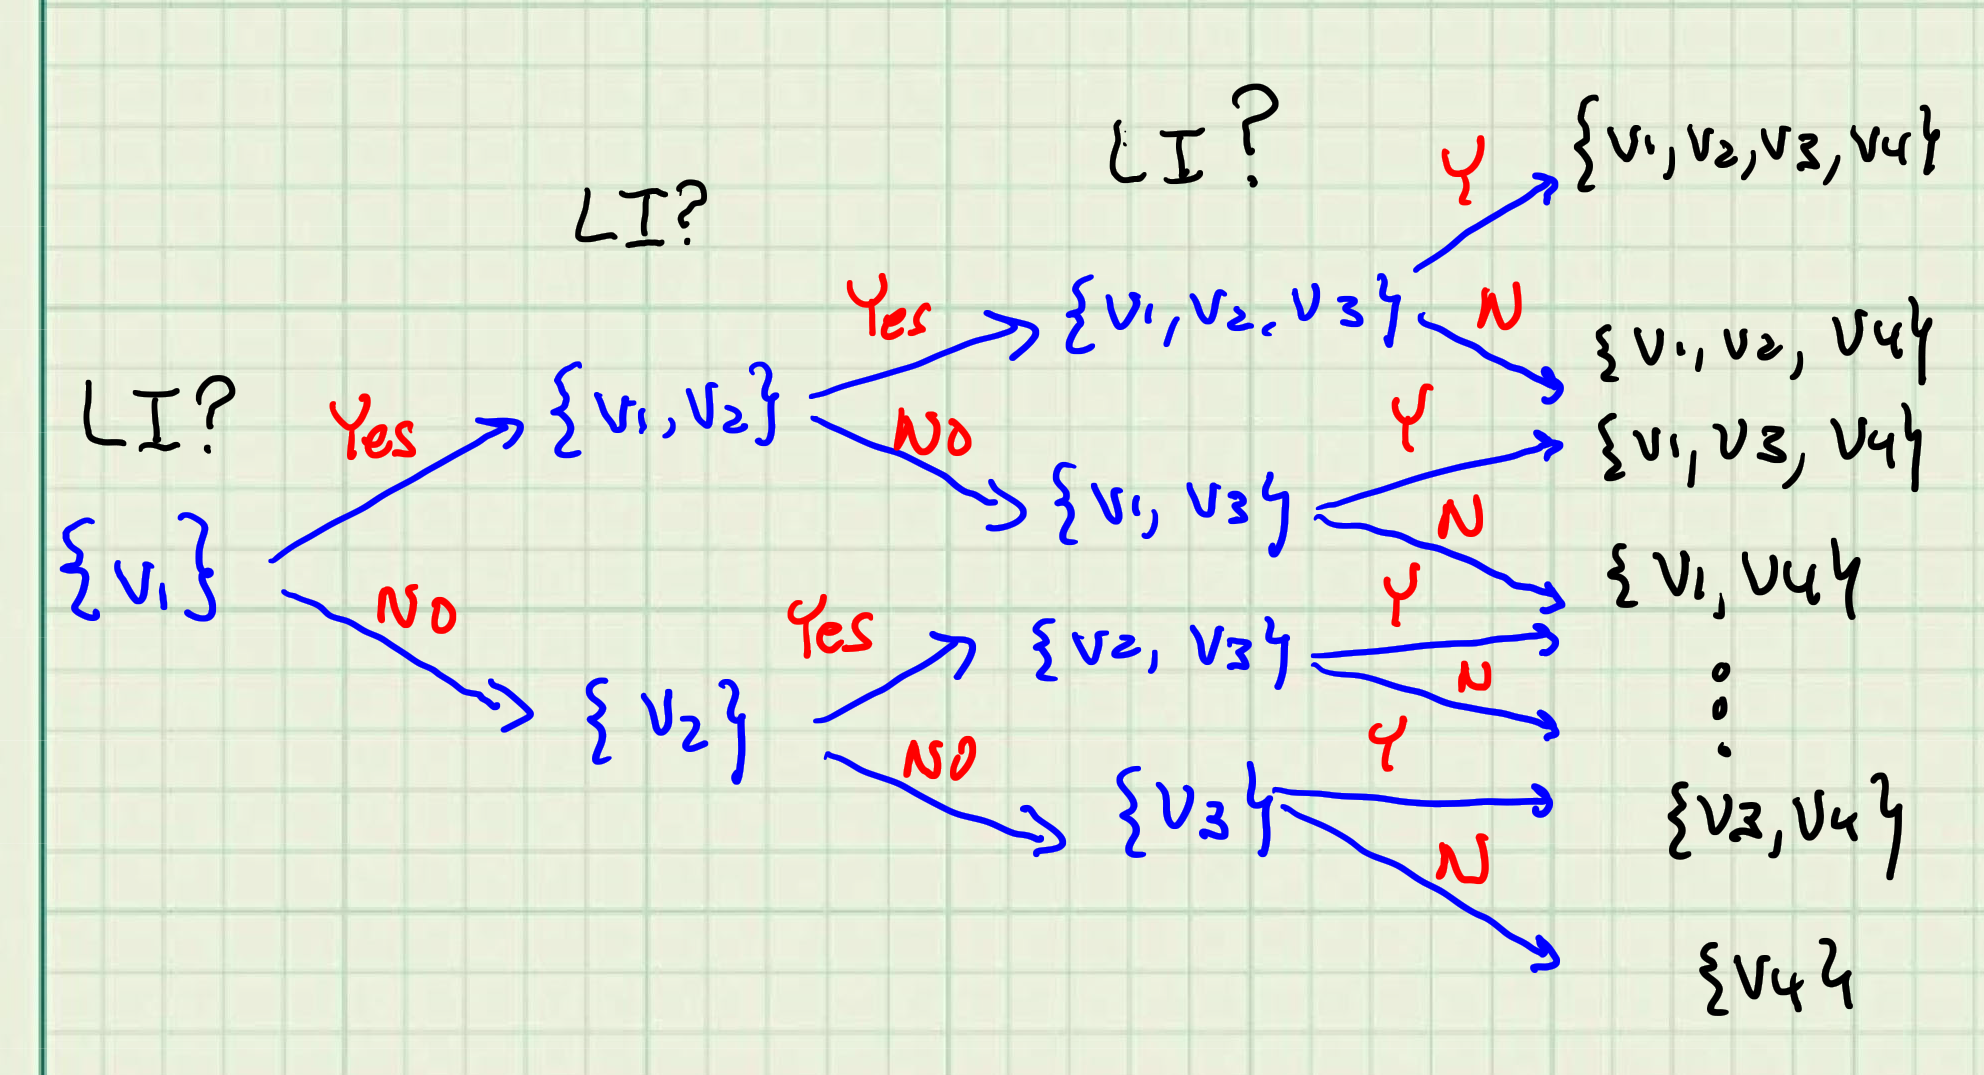
\includegraphics[width=0.88\columnwidth]{Chap07VectorSpaceRnPart1/NumberLinearIndependentVectorsInSet.png}%
\caption[]{Checking linear independence from left to right. You could also start from the right and go to the left, or you could start in the middle and proceed to the two ends. You just need to do an organized search of the vectors!}
    \label{fig:NumberLinearlyIndependentVectors}
\end{figure}

In fact there is. As illustrated in Fig.~\ref{fig:NumberLinearlyIndependentVectors}, we can start from left to right and ask, is the set $\{v_1\}$ linearly independent? If it is, keep $v_1$ and if not, discard it (meaning, in this case, $v_1$ was the zero vector). For the sake of argument, let's suppose that $v_1 \neq 0$ and hence we keep it. Next, we ask, is the set $\{ v_1, v_2\}$ linearly independent? If not, then $v_2$ is a linear combination of $v_1$ and we discard it, otherwise, we keep it. For the sake of argument, let's suppose that $v_2$ is a linear combination of $v_1$ and hence we discard it. We next ask, is the set $\{ v_1, v_3\}$ linearly independent? Let's say it is, and then we would ask if the set  $\{ v_1, v_3, v_4\}$ is linearly independent, etc. In the end, we have built the largest set of linearly independent vectors from the given set and we can ask, how many elements does it contain? 

\vspace*{.5cm}


\begin{tcolorbox}[title=\textbf{\large Number of Linearly Independent Vectors in  a Finite Set}] 
The following statements are equivalent:
\begin{itemize}
    \item One can divide the set of vectors in $\real^n$
\begin{equation}
\label{eq:VectorsFiniteList} v_1=\begin{bmatrix} a_{11} \\ a_{21}\\ \vdots \\ a_{n1} \end{bmatrix}, v_2=\begin{bmatrix} a_{12} \\ a_{22}\\ \vdots \\ a_{n2} \end{bmatrix}, ..., v_m=\begin{bmatrix} a_{1m} \\ a_{2m}\\ \vdots \\ a_{nm} \end{bmatrix}
\end{equation}
into $k$ linearly independent vectors and $m-k$ vectors that are linearly dependent on them.
\item The matrix 
\begin{equation}
\label{eq:MatrixFromLinearIndependence_IndepColumns}    
A=\left[\begin{array}{cccc} a_{11}& a_{12}& \cdots & a_{1m} \\
 a_{21}& a_{22}& \cdots & a_{2m}  \\
 \vdots & \vdots&  \ddots & \vdots \\
 a_{n1}& a_{n2}& \cdots & a_{nm} 
 \end{array}\right]
 \end{equation}
 has $k$ linearly independent columns and $m-k$ columns that are linearly dependent on them.
 \item Let $P \cdot \left(A^\top A \right) = L \cdot U$ be an LU Factorization of $A^\top A$. Then $U$ has $k$ linearly independent columns and $m-k$ dependent columns. Because $U$ is triangular, as in Example~\ref{ex:LinearIndep02}, checking linear independence is much easier than for the original matrix $A$.

\end{itemize}

\end{tcolorbox}

\begin{example} 
\label{ex:WithoutSemiProtip01} How many columns of the matrix 
\begin{equation}
\label{eq:WowCanWeAnalyzeThis}
A=\left[
\begin{array}{rrrrr}
-0.2 & -0.2 & -0.4 & 0.3 & 0.3 \\
0.3 & 1.0 & -0.1 & -1.1 & -1.7 \\
0.7 & -1.9 & 1.5 & -0.0 & -3.0 \\
0.9 & -1.0 & -0.7 & 0.6 & -1.8 \\
-0.5 & 0.8 & -1.1 & -0.5 & -0.5 \\
-2.0 & -0.9 & -0.5 & 0.2 & 0.3 \\
-1.0 & 0.6 & 0.7 & -0.9 & 0.2
\end{array}
\right]_{7 \times 5}
\end{equation}
are linearly independent? Doing this as shown in Fig.~\ref{fig:NumberLinearlyIndependentVectors} would be painful. 
\end{example}

\textbf{Solution:} We turn to Julia and perform the LU Factorization: $\mathbf{P \cdot (A^\top \cdot A) = L \cdot U }$, for which we only report the upper triangular matrix
\begin{equation}
U=\left[
\begin{array}{rrrrr}
6.680 & -1.090 & 1.320 & 0.900 & -4.840 \\
0.000 & 7.282 & -1.965 & -2.733 & 4.400 \\
0.000 & 0.000 & 4.069 & -1.525 & -0.506 \\
0.000 & 0.000 & 0.000 & 3.124 & 9.371 \\
0.000 & 0.000 &  0.000 & 0.000 &  0.000 
\end{array}
\right]_{5 \times 5} = \left[
\begin{array}{rrrrr}
u_1 & u_2 & u_3 & u_4 & u_5
\end{array}
\right]_{5 \times 5},
\end{equation}
where we have labeled its columns as $u_1 \ldots u_5$. Working from left to right with the columns of $U$, we have that because $u_1 \neq 0_{5 \times 1}$, the set $\{ u_1\}$ is linearly independent. We next check the set $\{ u_1, u_2\}$. To emphasize the beauty of the triangular structure in $U$, we check if there exist non-trivial solutions to 
$$\alpha_1 u_1 + \alpha_2 u_2 = \left[ \begin{array}{rr}
6.680 & -1.090  \\
0.000 & 7.282 \\
0.000 & 0.000 \\
0.000 & 0.000  \\
0.000 & 0.000 
\end{array} \right] \left[
\begin{array}{r} \alpha_1 \\ \alpha_2 \end{array}
\right] = \left[ \begin{array}{r}
0.0 \\0.0\\0.0\\0.0\\0.0
\end{array} \right]. $$
There answer is clearly no\footnote{There are three rows of zeros. Hence, starting from the second row, back substitution provides that the unique answer is zero}, the unique solution is $\alpha_1=0$ and $\alpha_2=0$, and thus $\{ u_1, u_2\}$ is linearly independent. The same reasoning works for  $\{ u_1, u_2, u_3\}$ and  $\{ u_1, u_2, u_3, u_4\}$. Indeed, we could have jumped straight to the set of vectors $\{ u_1, u_2, u_3, u_4\}$ because checking its linear independence comes down to looking for solutions to 
$$ \left[
\begin{array}{rrrrr}
\boxed{6.680} & -1.090 & 1.320 & 0.900 \\
0.000 & \boxed{7.282} & -1.965 & -2.733 \\
0.000 & 0.000 & \boxed{4.069} & -1.525  \\
0.000 & 0.000 & 0.000 & \boxed{3.124}  \\
0.000 & 0.000 &  0.000 & 0.000
\end{array}
\right] \left[
\begin{array}{r} \alpha_1 \\ \alpha_2  \\ \alpha_3 \\ \alpha_4\end{array}
\right]=  \left[ \begin{array}{r}
0.0 \\0.0\\0.0\\0.0\\0.0
\end{array} \right].$$
Ignoring the final row of zeros, we really have a square triangular system with a non-zero diagonal, hence the trivial solution $\alpha_1=\alpha_2=\alpha_3=\alpha_4=0$ is, in fact, the unique solution, proving linear independence.\\

What about $\{ u_1, u_2, u_3, u_4, u_5\}$? The answer is no, and to see this we note that 
\begin{align*} \alpha_1 u_1 +  \alpha_2 u_2 +  \alpha_3 u_3 + \alpha_4 u_4 + \alpha_5 u_5 &= 0_{5\times 1} \\
& \Updownarrow\\
\alpha_1 u_1 +  \alpha_2 u_2 +  \alpha_3 u_3 + \alpha_4 u_4 &= -\alpha_5 u_5
\end{align*}
Writing down this equation yields
$$\left[
\begin{array}{rrrrr}
\boxed{6.680} & -1.090 & 1.320 & 0.900 \\
0.000 & \boxed{7.282} & -1.965 & -2.733 \\
0.000 & 0.000 & \boxed{4.069} & -1.525  \\
0.000 & 0.000 & 0.000 & \boxed{3.124}  \\
0.000 & 0.000 &  0.000 & 0.000
\end{array}
\right] \left[
\begin{array}{r} \alpha_1 \\ \alpha_2  \\ \alpha_3 \\ \alpha_4\end{array}
\right]= - \left[ \begin{array}{r}
-4.840  \\4.400\\-0.506\\9.371\\ 0.000
\end{array} \right]  \alpha_5.
$$
If we set $\alpha_5=-1$, for example, and once again ignore the bottom row of zeros because they do not affect the solution of the equations, we can solve the resulting triangular system of equations for $\alpha_1$ through $\alpha_4$, giving us a non-trivial solution to $\alpha_1 u_1 + \cdots + \alpha_5 u_5=0$. Hence,  $\{ u_1, u_2, u_3, u_4, u_5 \}$ is linearly dependent. 
\Qed

\vspace*{0.5cm}
\textbf{Yes, the triangular structure of $U$ is very helpful, but it still requires a lot of work to check for solutions. Is there anything like our \textcolor{red}{\bf Pro-Tip} for linear independence that we can apply for counting the maximum number of linearly independent vectors?}


\vspace*{.2cm}

\begin{tcolorbox}[sharp corners, colback=green!30, colframe=green!80!blue,
title=\textbf{ {\Large \textcolor{red}{\bf Uber} Pro-Tip:} \large Number of Linearly Independent Vectors via an Enhanced LU Factorization}]
Assume that a set of vectors in \eqref{eq:VectorsFiniteList} have been stacked to form the columns of an $n \times m$ matrix $A$ as in \eqref{eq:MatrixFromLinearIndependence_IndepColumns}, or that the matrix $A$ has been given to us directly. \textbf{Fact:} The matrix $A^\top \cdot A$ always has an \textbf{LDLT Factorization}
\begin{equation}
    \label{eq:LDLTfactorization}
    P\cdot A^\top \cdot A \cdot P^\top = L\cdot D \cdot L^\top,
\end{equation}
where
\begin{itemize}
    \item $P$ is a (row) permutation matrix;
    \item $P^\top$, the transpose of $P$, permutes the columns of $A$;
    \item $L$ is uni-lower triangular and $L^\top$, the transpose of $L$, is therefore uni-upper triangular; and
    \item $D$ is diagonal and has non-negative entries.
\end{itemize}
\textcolor{red}{\bf Moreover,}
\begin{itemize}
    \item \textcolor{red}{\bf the number of linearly independent columns of $A$ is equal to the number of non-zero entries on the diagonal of $D$;} and, if we denote this number by $k$,
    \item  \textcolor{red}{\bf then for the version of the LDLT given below, the first $k$-columns of $A \cdot P^\top$ are linearly independent, and the remaining $(m-k)$-columns (if any) are linearly dependent on the first $k$ columns.} 
    \item Because the columns of $A\cdot P^\top$ are simply the columns of $A$ permuted by $P^\top$ (that is, re-ordered by the permutation matrix), \textcolor{red}{\bf the first $k$-columns of $A \cdot P^\top$ provide a selection of linearly independent columns of $A$}.
\end{itemize}

\end{tcolorbox}
\vspace*{.2cm}

The algorithm for LDLT Factorization is derived in Chap.~\ref{sec:LUsymmetric}, in case you are curious. You are not responsible for its derivation.

\vspace*{.2cm} 
\textbf{Remarks:} (Optional Read) The LDLT factorization may look intimidating, but once you realize that $U:=D \cdot L^\top$ is upper triangular, this is really a refined LU Factorization that is possible for matrices of the form $A^\top \cdot A$. The name \textcolor{blue}{\bf LDLT Factorization} comes from $L\cdot D \cdot L^\top$, where the last \textcolor{blue}{\bf T} stands for transpose. It is also called a \textbf{Cholesky Factorization}. Whatever you call it, it is simply our well known LU Factorization with $U$ in the special form  $U:=D \cdot L^\top$, which is possible for special kinds of matrices of the form $A^\top \cdot A$. \\

Recalling that the matrix transpose of a product is the product \textbf{in reverse order} of the matrix transposes, we check that
\begin{align*}
   \left(P\cdot A^\top \cdot A \cdot P^\top \right)^\top &= \left(P^\top \right)^\top \cdot \left(A \right)^\top \cdot \left(A^\top\right)^\top \cdot  \left(P \right)^\top\\
   &= P\cdot A^\top \cdot A \cdot P^\top,
\end{align*}
once one notes that $\left(A^\top\right)^\top =A$ and $\left(P^\top \right)^\top=P$. Hence $P\cdot A^\top \cdot A \cdot P^\top$ is symmetric. Without the $P^\top$ on the right, the term $P\cdot A^\top \cdot A$ alone would not be symmetric in general. A similar computation shows that $L\cdot D \cdot L^\top$ is also symmetric. \Qed

\vspace*{.2cm}
\textbf{Here is the Julia code for computing the LDLT Factorization:}
\begin{lstlisting}[language=Julia,style=mystyle]
# the LDLT factorization is a special LU Factorization for M=A'A
# P A' A P' = L D L', L unitriangular, D diagonal with non-negative entries, P permutation matrix
# the P' on the right does column permutations to maintain the symmetry of A'*A
#
function ldlt(A::Array{<:Number, 2})
    epsilon=1e-12
    M=A'*A
    n,m= size(A)
    Areduced = deepcopy(M)
    L = Array{Float64,2}(undef, m, 0)
    Id=zeros(m,m) + I
    P=deepcopy(Id)
    # could make D a vector for efficiency
    D=zeros(m,m)
        for i = 1:m
            # move the biggest entry to the pivot position
            ii=argmax( diag(Areduced[i:m,i:m]) );
            mrow=ii[1]+(i-1) 
            if ~(i==mrow)
                # row permuation
                P[[i,mrow],:]=P[[mrow,i],:];  
                # row and column permutation
                Areduced[[i,mrow],:]=Areduced[[mrow,i],:];
                Areduced[:,[i,mrow]]=Areduced[:,[mrow,i]];
            end
            if i>1
                L[[i,mrow],:] = L[[mrow,i],:];             
            end
            pivot=Areduced[i,i]
            if ~isapprox(pivot,0, atol=epsilon)
                D[i,i]=pivot
                C=Areduced[:,i]/pivot #normalize all entires by C[i]
                L=[L C]
                Areduced=Areduced-C*pivot*C'   
            else
                # Remainder of factorization is trivial
                L=[L Id[:,i:m]]
                break
            end 
        end
     diagD=diag(D)
return L, P, D, diagD
end
\end{lstlisting}

\vspace*{.2cm}

\begin{example} 
\label{ex:SemiProtip01} We revisit Example~\ref{ex:WithoutSemiProtip01}: how many columns of the matrix 
\begin{equation}
\label{eq:WowCanWeAnalyzeThis00}
A=\left[
\begin{array}{rrrrr}
-0.2 & -0.2 & -0.4 & 0.3 & 0.3 \\
0.3 & 1.0 & -0.1 & -1.1 & -1.7 \\
0.7 & -1.9 & 1.5 & -0.0 & -3.0 \\
0.9 & -1.0 & -0.7 & 0.6 & -1.8 \\
-0.5 & 0.8 & -1.1 & -0.5 & -0.5 \\
-2.0 & -0.9 & -0.5 & 0.2 & 0.3 \\
-1.0 & 0.6 & 0.7 & -0.9 & 0.2
\end{array}
\right]_{7 \times 5}
\end{equation}
are linearly independent?
\end{example}

\textbf{Solution:} We turn to Julia and perform the LDLT Factorization: $\mathbf{P \cdot A^\top \cdot A \cdot P^\top = L \cdot D \cdot L^\top}$, for which we report the diagonal of $D$
\begin{equation}
{\rm diag}(D) = \left[
\begin{array}{ccccc}
\BLUE 15.6 & \BLUE 5.2 & \BLUE 4.4 & \BLUE 2.3 & \RED 0.000 \end{array}
\right]_{1 \times 5}
\end{equation}

Because there are four non-zero entries on the diagonal of $D$,  we conclude that $A$ has four linearly independent columns.
\Qed


\vspace*{.5cm}

\begin{example} 
\label{ex:SemiProtip02} How many columns of the matrix 
\begin{equation}
A=\left[
\begin{array}{rrrrrr}
-0.2 & -0.2 & -0.4 & 0.3 & 0.3 & -0.5 \\
0.3 & 1.0 & -0.1 & -1.1 & -1.7 & 0.1 \\
0.7 & -1.9 & 1.5 & -0.0 & -3.0 & 0.3 \\
0.9 & -1.0 & -0.7 & 0.6 & -1.8 & -0.2 \\
-0.5 & 0.8 & -1.1 & -0.5 & -0.5 & -1.3 \\
-2.0 & -0.9 & -0.5 & 0.2 & 0.3 & -3.2 \\
-1.0 & 0.6 & 0.7 & -0.9 & 0.2 & -0.6 \\
\end{array}
\right]_{7\times 6}
\end{equation}
are linearly independent? \textcolor{blue}{Which ones are they?} 
\end{example}

\vspace*{0.2cm}

\textbf{Solution:}  We turn to Julia and perform the LDLT Factorization: $\mathbf{P \cdot A^\top \cdot A \cdot P^\top = L \cdot D \cdot L^\top}$, for which we report the diagonal of $D$
\begin{equation}
{\rm diag}(D)=\left[
\begin{array}{cccccc}
\BLUE  15.6 & \BLUE  12.6 & \BLUE  3.6 & \BLUE  2.6  & \RED 0.0 & \RED 0.0 
\end{array}
\right]_{1\times 6}
\end{equation}
which has four non-zero elements. We conclude that $A$ has four linearly independent columns. \\

We next compute
\begin{equation}
A \cdot P^\top=\left[
\begin{array}{rrrrrr}
0.3 & -0.5 & -0.4 & 0.3 & \RED -0.2 & \RED -0.2 \\
-1.7 & 0.1 & -0.1 & -1.1 & \RED 0.3 & \RED 1.0 \\
-3.0 & 0.3 & 1.5 & 0.0 & \RED 0.7 &\RED -1.9 \\
-1.8 & -0.2 & -0.7 & 0.6 & \RED 0.9 & \RED -1.0 \\
-0.5 & -1.3 & -1.1 & -0.5 & \RED -0.5 &\RED 0.8 \\
0.3 & -3.2 & -0.5 & 0.2 & \RED -2.0 &\RED -0.9 \\
0.2 & -0.6 & 0.7 & -0.9 & \RED -1.0 &\RED 0.6 \\
\end{array}
\right]
\end{equation}
and conclude that the first four columns of $A \cdot P^\top$ are linearly independent and the last two columns are linearly dependent on the first four. \\

Here, we can see that the four linearly independent columns correspond to columns 3, 4, 5, and 6 of $A$, while columns 1 and 2 of $A$ can be written as a linear combination of columns 3, 4, 5, and 6. Indeed, one can show
\begin{equation}
\left[
\begin{array}{rrrr}
0.3 & -0.5 & -0.4 & 0.3 \\
-1.7 & 0.1 & -0.1 & -1.1 \\
-3.0 & 0.3 & 1.5 & 0.0 \\
-1.8 & -0.2 & -0.7 & 0.6 \\
-0.5 & -1.3 & -1.1 & -0.5 \\
0.3 & -3.2 & -0.5 & 0.2 \\
0.2 & -0.6 & 0.7 & -0.9 \\
\end{array}
\right] \left[
\begin{array}{rr}
-0.33 & 0.33 \\
0.67 & 0.33 \\
-0.33 & -0.67 \\
0.33 & -1.33 \\
\end{array}
\right] = \left[
\begin{array}{rr}
-0.2 & -0.2 \\
0.3 & 1.0 \\
0.7 & -1.9 \\
0.9 & -1.0 \\
-0.5 & 0.8 \\
-2.0 & -0.9 \\
-1.0 & 0.6 \\
\end{array}
\right].
\end{equation}
 \Qed


\vspace*{.2cm}

\begin{tcolorbox}[title=\textbf{Identifying the Linearly Independent Vectors}]
 Is there a simple way to look at the data from the LDLT Factorization of $A^\top A$ and find a specific choice of columns of $A$ to form a linearly independent set? \textcolor{blue}{\bf Yes!} Here is the permutation matrix
\begin{equation}
P= \left[
\begin{array}{cccccc}
0.0 & 0.0 & 0.0 & 0.0 & 1.0 & 0.0 \\
0.0 & 0.0 & 0.0 & 0.0 & 0.0 & 1.0 \\
0.0 & 0.0 & 1.0 & 0.0 & 0.0 & 0.0 \\
0.0 & 0.0 & 0.0 & 1.0 & 0.0 & 0.0 \\
1.0 & 0.0 & 0.0 & 0.0 & 0.0 & 0.0 \\
0.0 & 1.0 & 0.0 & 0.0 & 0.0 & 0.0 \\
\end{array}
\right]
\end{equation}
for Example~\ref{ex:SemiProtip02}.
We see that, starting with the first row of $P$, the ones are in columns $\{5, 6, 3, 4, 1, 2 \}$, that is,
\begin{center}
 $P_{15}=1.0$, $P_{26}=1.0$, $P_{33}=1.0$, $P_{44}=1.0$, $P_{51}=1.0$ and $P_{62}=1.0$.   
\end{center} From this information, we can conclude that if we denote the columns of $A$ as $A=\left[\begin{array}{cccccc} A_1 & A_2 & A_3 & A_4 & A_5 & A_6\end{array} \right]$, then 
$$A \cdot P^\top = \left[\begin{array}{cccccc} A_5 & A_6 & A_3 & A_4 & A_1 & A_2 \end{array}\right]. $$
Since we know that $A \cdot P^\top$ has four linearly independent columns, we conclude that columns 
$$\{\begin{array}{cccc} A_5 & A_6 & A_3 & A_4  \end{array} \} $$
of $A$ are linearly independent.\\

You have to admit, it's pretty cool to do the analysis in this manner. 
\end{tcolorbox}

\textbf{Looking Ahead:} We will later have a very nice name for the number of linearly independent vectors in a set of vectors: the \textbf{dimension of $\spanof{v_1, v_2, \dots, v_m}$} For now, we're just counting the number of linearly independent vectors.\\

\vspace*{.2cm}



\section{Attractive Test for Linear Combinations}
\label{sec:AttractiveTestLinearCombination}

\begin{tcolorbox}[sharp corners, colback=green!30, colframe=green!80!blue,
title=\textbf{Pro Tip! Linear Combination or Not?}]
\textbf{Fact:} A vector $v_0\in \real^n$ can be written as a linear combination of $\{v_1, \ldots, v_m\} \subset \real^n$  if, and only if, the set $\{v_0, v_1, \ldots, v_m\}$ has the same number of linearly independent vectors as $\{v_1, \ldots, v_m\}$.\\

Applying this to determining if a linear system of equations $Ax=b$ has a solution, we first define $A_{\rm e} :=\left[A~~ b \right]$ by appending $b$ to the columns of $A$. Then we do the corresponding LDLT Factorizations
\begin{itemize}
    \item $P \cdot \left(A^\top \cdot A \right)\cdot P^\top = L \cdot D \cdot L^\top$
    \item $P_{\rm e} \cdot \left(A_{\rm e}^\top \cdot A_{\rm e}  \right) \cdot P^\top_{\rm e} = L_{\rm e} \cdot D_{\rm e} \cdot L^\top_{\rm e} $.
\end{itemize}

\textbf{Fact:}  $Ax=b$ has a solution if, and only if, $D$ and $D_{\rm e}$ have the same number of non-zero entries on their diagonals.\\

Why? We know that $Ax=b$ has a solution if, and only if, $b$ is a linear combination of the columns of $A$. That is, $A$ and $A_e:=[A~~b]$ must have the same number of linearly independent columns.\\

\textbf{(Optional Remark):} You get the same result by defining $A_{\rm e} :=\left[b~~ A \right]$; in fact, you can insert $b$ anywhere you want, even in the middle of the columns of $A$.
\end{tcolorbox}

\vspace*{.5cm}

\begin{example} 
\label{ex:LinearCombProTip01} We consider a rectangular system that is on the edge  of what we would like to analyze by hand,
\begin{equation}
    \label{eq:LinearCombProTip01Axequalsb}
\underbrace{ \left[
\begin{array}{rrr}
\begin{array}{ccc}
3.5 & 1.0 & 5.0 \\
5.0 & 2.0 & 6.0 \\
6.5 & 3.0 & 7.0 \\
8.0 & 4.0 & 8.0 \\
\end{array}
\end{array}
\right]}_{A} \underbrace{ \left[
\begin{array}{r}
x_1 \\
x_2 \\
x_3\\
\end{array}
\right]}_{x} = 
\underbrace{ \left[
\begin{array}{r}
4.0 \\
4.0 \\
4.0 \\
4.0 \\
\end{array}
\right]}_{b}.
\end{equation}
Does it have a solution? 
\end{example}

\textbf{Solution:} We seek to determine if \eqref{eq:LinearCombProTip01Axequalsb} will have a solution. We do the indicated LDLT Factorizations 
$$P \cdot \left(A^\top A \right) \cdot P^\top = L \cdot D \cdot L^\top~~\text{and}~~
 P_{\rm e} \cdot \left([A~~b]^\top [A~~b]  \right)\cdot  P_{\rm e}^\top = L_{\rm e}  \cdot  D_{\rm e} \cdot L_{\rm e}^\top  $$
and report the diagonals of $D$ and $D_e$ as row vectors
\begin{align}
    \label{eq:DiagOfU}
{\rm diag}(D)&= \left[
\begin{array}{ccc}
174.0 & 1.8 & 0.0 \\
\end{array}
\right]_{1 \times 3} \\
{\rm diag}(D_e)&= 
\left[
\begin{array}{cccc}
174.0 & 1.8 & 0.0 & 0.0  \\
\end{array}
\right]_{1 \times 4}.
  \label{eq:DiagOfUe}
\end{align}
Based on the above, we see that $A$ and $[A~~b]$ have the same number of linearly independent columns. Hence, $b$ is a linear combination of the columns of $A$ and therefore \eqref{eq:LinearCombProTip01Axequalsb} has a solution. In fact, one can compute a solution is 
\begin{equation}
\label{eq:OneSolutionOrUniqueSolution}
x=\left[
\begin{array}{r}
0.0 \\
-1.0 \\
1.0 \\
\end{array}
\right].
\end{equation}\\

We now change the vector $b$ to 
$$
\left[
\begin{array}{r}
20.0 \\
11.0 \\
12.0 \\
14.0 \\
\end{array}
\right],
$$
and repeat the analysis, giving 
\begin{align}
    \label{eq:DiagOfUB}
{\rm diag}(D)&= \left[
\begin{array}{ccc}
174.0 & 1.8 & 0.0 \\
\end{array}
\right]_{1 \times 3} \\
  \label{eq:DiagOfUeC}
{\rm diag}(D_e)&= 
\left[
\begin{array}{cccc}
861.0 & 28.3 & 0.5 & 0.0 \\
\end{array}
\right]_{1 \times 4}.
\end{align}
This time, the analysis shows that $[A~~b]$ has one more linearly independent column than $A$, and hence $b$ is linearly independent of the columns of $A$. We conclude, therefore, that the new system of linear equations does not have a solution. 
\Qed


\section{Existence and Uniqueness of Solutions to Ax=b}

In Chapter~\ref{sec:UniquenessSolutions}, we showed that $Ax=b$ has a solution if, and only if, $b$ is a linear combination of the columns of $A$. Here, we will show that uniqueness of a solution follows from the columns of $A$ being linearly independent. \textbf{When both of these conditions hold, we have existence and uniqueness of solutions.} \\

Let $A$ be an $n \times m$ matrix, not necessarily square, and consider 
\begin{equation}
\label{eq:UniquenessSolutionsNonsquare}    
 \underbrace{\left[\begin{array}{cccc} a_{11}& a_{12}& \cdots & a_{1m} \\
 a_{21}& a_{22}& \cdots & a_{2m}  \\
 \vdots & \vdots&  \ddots & \vdots \\
 a_{n1}& a_{n2}& \cdots & a_{nm} 
 \end{array}\right] }_{A} \underbrace{\left[ \begin{array}{c} x_1 \\ x_2 \\
\vdots \\ x_m   \end{array} \right]}_{x} = \underbrace{\left[ \begin{array}{c} b_1 \\ b_2 \\ \vdots \\ b_n  \end{array} \right]}_{b}.
\end{equation}

Suppose that $\overline{x}$ satisfies $A \overline{x} =b$, which is the same thing as saying $\overline{x}$ is a solution of $Ax=b$. Suppose also that $\doverline{x}$ satisfies $A \doverline{x} =b$. We give conditions that guarantee
$ \doverline{x} =\overline{x}.$

\begin{tcolorbox}

If both $\overline{x}$ and  $\doverline{x}$ satisfy $Ax=b$, we have that
$$A\doverline{x} - A \overline{x} = A \left(\doverline{x} - \overline{x} \right) =  b - b =0.$$
We define $\alpha:=\doverline{x} - \overline{x}$ and write out its components as
$$\alpha := \left[ \begin{array}{c} \alpha_1 \\ \alpha_2 \\ \vdots \\ \alpha_m  \end{array} \right] $$
Expanding the expression $A \alpha = 0$ in terms of the columns of $A$ and the components of the vector $\alpha$ gives
\begin{equation}
    \label{eq:UniquenessSolutionsNonsquare_02}
\alpha_1 \underbrace{\begin{bmatrix} a_{11} \\ a_{21}\\ \vdots \\ a_{n1} \end{bmatrix}}_{a^{\rm col}_1}+ \alpha_2 \underbrace{\begin{bmatrix} a_{12} \\ a_{22}\\ \vdots \\ a_{n2} \end{bmatrix}}_{a^{\rm col}_2} + \cdots + \alpha_m \underbrace{\begin{bmatrix} a_{1m} \\ a_{2m}\\ \vdots \\ a_{nm} \end{bmatrix}}_{a^{\rm col}_m} = \begin{bmatrix} 0 \\ 0\\ \vdots \\ 0 \end{bmatrix}.
\end{equation}
We know that $\alpha_1=0, \alpha_2=0, \ldots, \alpha_m=0$ is the unique solution to 
$$\alpha_1 a^{\rm col}_1 + \alpha_2 a^{\rm col}_2 + \ldots \alpha_m a^{\rm col}_m = 0,$$
if and only if, the vectors $\{a^{\rm col}_1, a^{\rm col}_2, \ldots, a^{\rm col}_m \} $ are linearly independent. Hence, if $Ax=b$ has a solution, it will be unique if, and only if, the columns of $A$ are linearly independent.

\end{tcolorbox}

\vspace*{.2cm}

\begin{tcolorbox}[sharp corners, colback=green!30, colframe=green!80!blue, title=\textbf{\large Existence and Uniqueness of Solutions to $Ax=b$}]
The following two statements are equivalent
\begin{enumerate}
\renewcommand{\labelenumi}{(\alph{enumi})}
\setlength{\itemsep}{.2cm}
\item The system of linear equations $Ax=b$ has a solution, and, it is unique.

\item $b$ is a linear combination of the columns of $A$, and, the columns of $A$ are linearly independent. 
\end{enumerate}

\textbf{Remark:} If $b$ is not a linear combination of the columns of $A$, then $Ax=b$ does not have a solution. If the columns of $A$ are not linearly independent, then if $Ax=b$ has one solution, it also has an infinite number of solutions. \\

\textbf{Remark:} Please return to Chapter~\ref{sec:WhatCanHappen} and re-work the examples using this knowledge. Our new results do not even require the system of equations to be square, and moreover, thanks to our Pro and Uber-Pro Tips, our results are not limited to a small number of equations that are amenable to hand calculations!
\end{tcolorbox}

\vspace*{.2cm}

\begin{example}
\label{eq:BigExampleRectangular}
Let's analyze an example that most of us could not get right if done by hand! We consider $Ax=b$, where
\begin{equation}
\label{eq:WowCanWeAnalyzeThis02}
A=\left[
\begin{array}{rrrrr}
-0.2 & -0.2 & -0.4 & 0.3 & 0.3 \\
0.3 & 1.0 & -0.1 & -1.1 & -1.7 \\
0.7 & -1.9 & 1.5 & -0.0 & -3.0 \\
0.9 & -1.0 & -0.7 & 0.6 & -1.8 \\
-0.5 & 0.8 & -1.1 & -0.5 & -0.5 \\
-2.0 & -0.9 & -0.5 & 0.2 & 0.3 \\
-1.0 & 0.6 & 0.7 & -0.9 & 0.2
\end{array}
\right]_{7 \times 5}\text{and}~~~b=\left[
\begin{array}{r}
-0.5 \\
0.1 \\
0.3 \\
-0.2 \\
-1.3 \\
-3.2 \\
-0.6
\end{array}
\right]_{7 \times 1}
\end{equation}
Does it have a solution? If it does, is it unique? 
\end{example}


\textbf{Solution:} We form $A^\top A$ and compute in Julia its LDLT Factorization  and report the diagonal of $D$ as a row vector
\begin{equation}
{\rm diag}(D) = \left[
\begin{array}{ccccc}
15.6 & 5.2 & 4.4 & 2.3 & 0.0\\
\end{array}
\right]_{1 \times 5}
\end{equation}
There is a single zero on the diagonal and four non-zero elements. Thus we know that exactly four of the five columns of $A$ are linearly independent. Hence, if there does exist a solution to $Ax=b$, it will not be unique.\\

Next, we form $A_e :=[A~~b]$ and compute in Julia the LDLT Factorization of $A_e^\top A_e$. We report the diagonal of $D_e$ written as a row vector
\begin{equation}
{\rm diag}(D_e)=\left[
\begin{array}{cccccc}
15.6 & 12.6 & 3.6 & 2.6 & 0.0 & 0.0 
\end{array}
\right]_{1 \times 6}
\end{equation}
and note that it also has four non-zero entries. We deduce that $b$ is a linear combination of the columns of $A$. Hence, the system of linear equations \eqref{eq:WowCanWeAnalyzeThis02} has a solution and it is not unique. Therefore, it has an infinite number of solutions!\\

We select a different right hand side for \eqref{eq:WowCanWeAnalyzeThis02} and report the key result of its LDLT Factorization,
\begin{equation}
\tilde{b} = \left[
\begin{array}{r}
0.6 \\
0.4 \\
0.9 \\
1.0 \\
0.8 \\
0.8 \\
0.9
\end{array}
\right] \implies{\rm diag}(\tilde{D}_e) =\left[
\begin{array}{cccccc}
15.6 & 5.2 & 1.2 & 2.3 & 0.9 & 0.0  \\
\end{array}
\right]_{1 \times 6}.
\end{equation}
This time ${\rm diag}(\tilde{D}_e)$ has five non-zero entries, whereas ${\rm diag}(D)$ had four non-zero entries.  Hence, $\tilde{b}$ is not a linear combination of the columns of $A$, and the system of equations, with this new right hand side, does not have a solution.
\Qed


\section{When are the Solutions to $Ax=b$ the same as the Solutions to $M \cdot A x = M \cdot b$?}

So far, we have seen two special cases of multiplying (both sides of) a set of equations on the LEFT by a matrix $M$ of compatible size. 
\begin{enumerate}
    \item[a)] In Chapter~\ref{sec:UtilityMatrixInverse}, we noted that if $A$ is invertible, then
    $$ A x = b \iff \underbrace{A^{-1} \cdot A}_{I} x =  A^{-1}  b \iff x =  A^{-1} b.$$

    \item[b)] In Chapter~\ref{sec:SolvingAxeqBviaLUrowPermutations}, for $P$ a permutation matrix, we noted that
    $$ Ax = b \iff P \cdot A x = P b,$$
    where we needed this result when applying the LU Factorization $P \cdot A = L \cdot U$ to solve $Ax = b$. 
\end{enumerate}
Here, we will generalize these two special cases to a more general situation of multiplying on the left by a size-compatible matrix $M$ that can be \textbf{rectangular}.\\

We assume that $A$ is $n \times m$ and $b$ is $m \times 1$. Then for any $p \times n$ matrix $M$, the matrix multiplications $M \cdot A$ and $M b$ both make sense. We now ask the question, for what matrices $M$ is it true that $Ax = b$ and $M \cdot A x = M b$ have the same solutions? It turns out that \textbf{linear independence} of the columns of $M$ is sufficient for this to hold.\\

To see this, we define $y = Ax - b$ and note that $x \in \real^m$ is a solution to $Ax=b$ if, and only if, $y = 0_{n \times 1}$; we have simply said that $Ax = b \iff Ax - b = 0_{n \times 1}$. Similarly, we note that $x \in \real^m$ is a solution to $M \cdot A x = M \cdot b$ if, and only if, $M y = 0_{p\times 1}$, which is because $M \cdot A x = M \cdot b \iff M \cdot(A x - b) = 0_{p \times 1}$. So far, so good. \\

Surprisingly, the proof is done! Why? From our proof of the Pro-Tip in Chapter~\ref{sec:ProofProTip}, we have that if the columns of $M$ are linearly independent, then 
$$y = 0_{n \times 1} \iff M ~y = 0_{ p \times 1}.$$
In other words, if the columns of $M$ are linearly independent, then $x$ is a solution of $Ax = b$ if, and only if, $x$ is a solution of  $M \cdot A x = M \cdot b$. \\

\textbf{What about the converse? (that is, the other direction?) } If $Ax=b$ and $M \cdot A x = M \cdot b$ have the same solutions, can we conclude that the columns of $M$ are linearly independent? In general, that statement is false. Consider, 
$$\underbrace{\left[
\begin{array}{cc}
1 & 0 \\
1 & 1\\
1 & 0 
\end{array}
\right] }_{A}  \begin{bmatrix}
    x_1 \\x_2
\end{bmatrix} =\underbrace{\begin{bmatrix}
    1\\0 \\1
\end{bmatrix} }_{b} \text{ and define } M := \left[
\begin{array}{ccc}
1 & 0 & 0\\
0 & 1 & 0\\
0 & 0  & 0
\end{array}
\right] \text{ so that } \underbrace{\left[ \begin{array}{cc}
1 & 0 \\
1 & 1\\
0 & 0 
\end{array}
\right] }_{M \cdot A}  \begin{bmatrix}
    x_1 \\x_2
\end{bmatrix} =\underbrace{ \begin{bmatrix}
    1\\0 \\0
\end{bmatrix} }_{M \cdot b}.$$
Then $x_1 = 1$, $x_2=-1$ is the unique solution to both systems of linear equations, but the columns of $M$ are not linearly independent because of the column of zeros. Finding a counterexample is how we go about showing something is false. 

\begin{remark} In Chapter~\ref{chap:NormRegression}, we will \textbf{deliberately} multiply both sides of an equation that has \textbf{no solutions} by a matrix with columns that are linearly \textbf{dependent} so as \textbf{to create a system of equations that has a unique solution.} It's kind of mind-blowing, we know! That's part of why Linear Algebra is so exciting! Like a good mystery novel, its plot has unexpected twists and turns. 
\end{remark}


\section{(Optional Read): Why LDLT and not Simply LU?}
\label{sec:WhyLDLT}
 This is intended for instructors! Why can't one simply use the LU Factorization to determine the number of linearly independent columns? Why must one use the LDLT Factorization? For those with a driving sense of curiosity or simply a high tolerance for pain, here is an example of a matrix $A$ where the number of non-zero elements on the diagonal of $U$ with a standard LU Factorization does not correspond to the number of linearly independent columns of $A$, where
$$P \cdot A^\top \cdot A = L \cdot U. $$
Consider
$$A=\left[
\begin{array}{ccc}
0 & 0 & 0\\
0 & 1 & 0\\
0 & 0 & 0
\end{array}
\right]. $$
$A$ is symmetric, meaning that $A^\top = A$. Moreover, you can check that $A^\top \cdot A = A$. The following is a valid LU Factorization with row permutations
$$ \underbrace{\left[
\begin{array}{ccc}
0 & 1 & 0\\
1 & 0 & 0\\
0 & 0 & 1
\end{array}
\right]}_{P} \cdot \underbrace{\left[
\begin{array}{ccc}
0 & 0 & 0\\
0 & 1 & 0\\
0 & 0 & 0
\end{array}
\right]}_{A^\top \cdot A} = \underbrace{\left[
\begin{array}{ccc}
1 & 0 & 0\\
0 & 1 & 0\\
0 & 0 & 1
\end{array}
\right]}_{L} \cdot  \underbrace{\left[ \begin{array}{ccc}
\boxed{0} & 1 & 0\\
0 & \boxed{0} & 0\\
0 & 0 & \boxed{0}
\end{array}
\right]}_{U}. $$
We see that $U$ has one linearly independent column (the same as $A$), while ${\rm diag}(U)$ has three zeros. Hence, the number of non-zero elements on the diagonal of $U$ does not always correspond to the number of linearly independent columns of $A$ and $U$. For the magicians, we note that the eigenvalue zero of $U$ has algebraic multiplicity three and geometric multiplicity two. When we include the necessary column permutations to maintain the symmetry of $P \cdot A^\top \cdot A \cdot P^\top$ at each step of the factorization, we avoid this problem because eigenvalues of symmetric matrices always have equal geometric and algebraic multiplicities. This fact is way beyond the scope of ROB 101.
\Qed

\section{(Optional Read): LU Factorization for Symmetric Matrices}
\label{sec:LUsymmetric}

Recall that a matrix $M$ is symmetric if $M^\top = M$. For such matrices, we seek to refine our way of computing the LU Factorization so that at each stage of the reduction, ${\rm Temp}_{k+1} = {\rm Temp}_{k}-C_k \cdot R_k$, we preserve the symmetry of the matrix. We will discover a condition that will allow us to write
\begin{equation}
    \label{eq:PMPtransFormLU}
     P \cdot M \cdot P^\top = L \cdot D \cdot L^\top, 
\end{equation}
where $P$ is a permutation matrix, $L$ is uni-lower triangular, and $D$ is a diagonal matrix. When we can accomplish such a factorization, it will follow that the number of linearly independent columns of $M$ is precisely equal to the number of non-zero elements on the diagonal of $D$. A useful application of this result would then be counting the number of linearly independent columns in a rectangular matrix $A$ by counting the number of linearly independent columns of $A^\top A$, which is always symmetric. \\

To build up our intuition, consider a $3 \times 3$ symmetric matrix
\begin{equation}
    \label{eq:SymmetricM}
  {\rm Temp}_{1}:= M= \left[\begin{array}{ccc} 
   a & b & c\\
   b & d & e\\
   c & e & f
   \end{array}\right],
\end{equation}
   which has six parameters.
If $a\neq 0$, our first step in constructing the LU Factorization is to define
\begin{equation}
    \label{eq:SymmetricM_LUStep1a}
   \tilde{C}_1= \left[\begin{array}{c} 
   a \\  b \\ c 
   \end{array}\right] \frac{1}{a}~~\text{and}~~\tilde{R}_1=\left[\begin{array}{ccc}
   a & b & c
   \end{array}\right],
\end{equation}
where we are using a bar over the extracted columns and rows to distinguish them from a slightly different definition we will give shortly. The symmetry in $\tilde{C}_1$ and $\tilde{R}_1$ is clearly visible and it comes from the symmetry in $M$.\\

We can take better advantage of the symmetry in $M$ if we define instead
\begin{equation}
    \label{eq:SymmetricM_LUStep1b}
   C_1= \left[\begin{array}{c} 
   a \\  b \\ c 
   \end{array}\right]\frac{1}{a}, ~D_{11}=a~~\text{and}~~R_1=C_1^\top.
\end{equation}
It follows that
\begin{equation}
    \label{eq:SymmetricM_LUStep1c}
   C_1 \cdot D_{11} \cdot C_1^\top = C_1 \cdot D_{11} \cdot R_1 = \tilde{C}_1 \cdot \tilde{R}_1.
\end{equation}
A nice property of $C_1 \cdot D_{11} \cdot C_1^\top$ is that it is clearly symmetric. Also, if we subtract one symmetric matrix from another, the result is another symmetric matrix, so the symmetry property propagates. In our case, we'd have something like
\begin{equation}
    \label{eq:SymmetricM_LUStep1d}
{\rm Temp}_{2} := M -C_1 \cdot D_{11} \cdot C_1^\top =\left[\begin{array}{ccc} 
   a & b & c\\
   b & d & e\\
   c & e & f
   \end{array}\right] - \left[\begin{array}{ccc} 
   a & b & c \medskip \\
   b & \frac{b^2}{a} & \frac{b c}{a} \medskip \\
   c & \frac{b c}{a} & \frac{c^2}{a}
   \end{array}\right] = \left[\begin{array}{ccc} 
   0& 0 & 0\\
   0 & \alpha & \beta\\
   0 & \beta & \gamma
   \end{array}\right].
\end{equation}
We let the reader fill in the values of $\alpha$, $\beta$, and $\gamma$ because all we care is that ${\rm Temp}_{2}$ is symmetric and we can repeat the process. \\

When doing the LU Factorization, there were two other cases to consider. One is when there is an entire column of zeros, as in 
\begin{equation}
    \label{eq:SymmetricM_Step2}
  {\rm Temp}_{1}:= M= \left[\begin{array}{ccc} 
   0 & 0 & 0\\
   0 & d & e\\
   0 & e & f
   \end{array}\right],
\end{equation}
so that $a=b=c=0$. Because of the symmetry in ${\rm Temp}_{1}$, if we have an entire column of zeros, we also have an entire row of zeros! When we had entire column of zeros, we defined
\begin{equation}
    \label{eq:SymmetricM_LUStep2a}
   \tilde{C}_1= \left[\begin{array}{c} 
   1 \\  0 \\ 0 
   \end{array}\right] ~~\text{and}~~\tilde{R}_1=\left[\begin{array}{ccc}
   a & b & c
   \end{array}\right]= \left[\begin{array}{ccc}
   0 & 0 & 0
   \end{array}\right],
\end{equation}
We can take better advantage of the symmetry if we instead  define
\begin{equation}
    \label{eq:SymmetricM_LUStep2b}
   C_1= \left[\begin{array}{c} 
   1 \\  0 \\ 0
   \end{array}\right], ~D_{11}=0~~\text{and}~~R_1=C_1^\top.
\end{equation}
It still follows that
\begin{equation}
    \label{eq:SymmetricM_LUStep2c}
   C_1 \cdot D_{11} \cdot C_1^\top = C_1 \cdot D_{11} \cdot R_1 = \tilde{C}_1 \cdot \tilde{R}_1,
\end{equation}
and ${\rm Temp}_{2} := M -C_1 \cdot D_{11} \cdot C_1^\top$ is once again symmetric, with the first column and first row identically zero, so the process continues. So far, no permutation matrices have shown up!\\

A permutation of rows is required when our matrix has a zero in the entry that is supposed to define the pivot, such as here,
\begin{equation}
    \label{eq:SymmetricMStep3}
  {\rm Temp}_{1}:= M= \left[\begin{array}{ccc} 
   0 & b & c\\
   b & d & e\\
   c & e & f
   \end{array}\right],
\end{equation}
where $a=0$. If $b\neq 0$, we would swap the first and second rows to arrive at
\begin{equation}
    \label{eq:SymmetricMStep4}
  P \cdot {\rm Temp}_{1}:=  \left[\begin{array}{ccc}
    b & d & e\\
   0 & b & c\\
   c & e & f
   \end{array}\right],
\end{equation}
where to swap the first two rows, we have 
\begin{equation}
    \label{eq:SymmetricMStep5}
P=\left[\begin{array}{ccc}
    0 & 1 & 0\\
   1 & 0 & 0\\
   0 & 0 & 1
   \end{array}\right]. 
  \end{equation}
 But, in \eqref{eq:SymmetricMStep4}, we have destroyed the symmetry of our matrix!
  
\begin{tcolorbox}[title=  \textbf{\RED \large Destroyed Symmetry!}]
 A key observation is that we can  \textcolor{red}{\bf RESTORE SYMMETRY} if we also swap the first and second columns,  like this,
 \begin{equation}
    \label{eq:SymmetricMStep4b}
  \left[\begin{array}{ccc}
    d & b & e\\
   b& 0 & c\\
   e & c & f
   \end{array}\right],
\end{equation}
but oops, we no longer have $b\neq 0$ at the pivot position. We've moved $d$, an element of the diagonal, to the pivot position. If we had instead swapped rows one and three, followed by a swap of columns one and three, we'd end up with $f$, another element of the diagonal, at the pivot position! Hence, if preserving symmetry is our goal, we need to look at the diagonal of ${\rm Temp_k}$ for a non-zero element, and then to a double swap, two rows and two columns, to move it to the pivot position and continue the algorithm. The swapping of the columns is achieved by multiplying ${\rm Temp_k}$ on the right (instead of the left, which we do for row swapping), and the required permutation matrix can be shown to be the transpose of the matrix used to do the row swapping! Go to Julia and play round with it. It'll be fun! \\

\textbf{For a general symmetric matrix, if we arrive at a step where $\mathbf{diag}( \mathbf{Temp}_\mathbf{k})$ is all zeros, then the algorithm fails} and we cannot factor $M$ as
in \eqref{eq:PMPtransFormLU}. A matrix that will lead to immediate failure is
 \begin{equation}
   \label{eq:SymmetricBadMatrix}
   M=\left[\begin{array}{cc}
    0 & 1\\
  1 & 0
   \end{array}\right].
\end{equation}
However, if $M=A^\top \cdot A$ for some matrix $A$, then $M$ is a \textit{positive semi-definite matrix}. For such matrices, $$\mathbf{diag}( \mathbf{Temp}_\mathbf{k}) =0 \iff \mathbf{Temp}_\mathbf{k} = 0,$$
in which case the algorithm can be completed as we did for the LDLT Factorization presented earlier.
\end{tcolorbox}  

\vspace*{0.5cm}

We give the resulting algorithm and then revisit a few of our previous examples. So that a novice user can play around and check whether or not $Q=P^\top$ and $U=D\cdot L^\top$, we compute the additional matrices. You are free to remove them. 

\vspace*{0.5cm}

\begin{lstlisting}[language=Julia,style=mystyle]
# LU Factorization for Symmetric Matrices
# P M P' = L D L', L unitriangular, D diagonal, P permutation matrix
#
function luJWGSymD(M::Array{<:Number, 2})
    epsilon=1e-12; K=100
    if isapprox(norm(M-M'),0, atol=epsilon)
        # M is indeed symmetric
        n, m = size(M)
        Areduced = deepcopy(M)
        L = Array{Float64,2}(undef, n, 0)
        # Could remove U for efficiency
        U = Array{Float64,2}(undef, 0, n)
        P=zeros(n,n) + I
        # Could remove Q for efficiency
        Q=zeros(n,n) + I 
        # could make D a vector for efficiency
        D=zeros(n,n)
        for i = 1:n
            C = Areduced[:,i] # i-th column
            R = C' # i-th row
            if maximum(abs.(C)) <= K*epsilon #column of zeros
                C=0.0*C; C[i]=1.0; R = 0.0*R
                U=[U;R];  
                L=[L C];
                D[i,i]=0.0
                Areduced=Areduced-C*R;
            else # move the biggest entry to the pivot position
                ii=argmax( abs.(diag(Areduced)) );
                nrow=ii[1] 
                P[[i,nrow],:]=P[[nrow,i],:];
                Q[:,[i,nrow]]=Q[:,[nrow,i]];      
                Areduced[[i,nrow],:]=Areduced[[nrow,i],:];
                Areduced[:,[i,nrow]]=Areduced[:,[nrow,i]];
                if i>1
                    L[[i,nrow],:] = L[[nrow,i],:];
                    U[:,[i,nrow]] = U[:,[nrow,i]];
                    d1=D[i,i];d2=D[nrow,nrow]
                    D[i,i]=d2;D[nrow,nrow]=d1                
                end
                C = Areduced[:,i] # i-th column
                R = C' # i-th row
                pivot = C[i];
                if isapprox(pivot,0, atol=epsilon)
                    if isapprox(norm(Areduced),0, atol=K*epsilon)
                        # Remainder of factorization is trivial
                        L=[L Id[:,i:m]]
                        # U=D*L'; Q=P'; # All matrices included for pedagogical reasons
                        return L, U, P, Q, D
                        break
                    else
                        println("Algorthm failed at step $i")
                        println("A symmetric factorization PMP' = L D L' is not possible.")
                        return -1.0
                        break
                    end
                else
                    D[i,i]=pivot
                    C=C/pivot #normalize all entires by C[i]
                    U=[U;R];  # could remove U for efficiency
                    L=[L C];
                    Areduced=Areduced-C*R;
                end
                Areduced[:,i]=0*Areduced[:,i]; Areduced[i,:]=0*Areduced[i,:];
          end 
    end
        # U=D*L'; Q=P'; # All matrices included for pedagogical reasons
        return L, U, P, Q, D
    else 
        println("Matrix is not symmetric")
        return 0.0
    end
end
\end{lstlisting}

\textbf{Why does the LDLT Factorization work for matrices of the form $A^\top \cdot A$?} The proof needs ideas from positive semi-definite matrices as presented in Appendix~\ref{sec:PosDefMatrices}. Here we'll sketch the proof assuming the material in the Appendix is known, which may help instructors using the book. We suppose that $M:={\rm Temp}_k$ is positive semi-definite and we arrive at a step of LDLT where the diagonal of $M$ consists only of zeros. We write the matrix as
$$ M=\left[ \begin{array}{cc} 0 & M_{12}\\ M_{12}^\top & M_{22} \end{array}  \right], $$ and note that $M_{22}$ must be positive semi-definite by the assumption on $M$. We claim that necessarily, $M_{12}=0$, the zero vector. To show this, we form the product
$$ x^\top M x = \left[ \begin{array}{cc} x_1 & x_2^\top \end{array} \right] \left[ \begin{array}{cc} 0 & M_{12}\\ M_{12}^\top & M_{22} \end{array} \right] \left[ \begin{array}{c}x_1 \\ x_2 \end{array}  \right] = 2 x_1 M_{12} x_2 + x_2^\top M_{22} x_2. $$
If $M_{12}\neq 0$, then there exists $x_2$ such that $ M_{12} x_2 < 0$. It follows that by taking $x_1>0$ sufficiently large, that
$$2 x_1 M_{12} x_2 + x_2^\top M_{22} x_2 <0, $$
which contradicts $M$ being positive semi-definite. This argument can be repeated. Applying it by induction to $M_{22}$, we arrive at $M$ is the zero matrix, which can be easily factored. Otherwise, at each step, we have non-zero elements on the diagonal of $M:={\rm Temp}_k$ and the LDLT Factorization can be continued. 

\section{Looking Ahead}

In the next Chapter, we show how to measure the ``length'' of a vector and use that to formulate the problem of finding approximate solutions to linear systems of equations that do not have exact solutions. At first blush, this seems like a strange thing to do. In real engineering, however, the data we collect is never exact. The data is perturbed by various sources of errors, from imprecision in our instruments, to the fact that experiments are hard to repeat! To get around this, we take many more measurements than we need, which gives us sets of what we call ``overdetermined equations,'' which means more equations than unknown variables. We seek to ``smooth'' or ``average'' out the measurement errors by finding approximate solutions so that $e:=Ax-b$, the error in the ``equation,'' is small. We measure the ``length of the error vector'' by a function called the ``Euclidean norm.''
